\documentclass[output=paper,modfonts,nonflat,newtxmath]{langsci/langscibook}
\author{Simone E. Pfenninger\affiliation{University of Salzburg}}
\title{Age meets multilingualism: Influence of starting age on L3 acquisition across different learner populations}
\abstract{This paper combines for the first time two major strands of multilingualism research, namely that of the role of starting age in (multiple) foreign language (FL) learning, and that of the influence of bilingualism and biliteracy on third language (L3) acquisition. I report on the results of a five-year longitudinal study in Switzerland, in which we assessed the English development of 636 secondary school students, who had all learned Standard German and French at primary school, but only half of whom had had English from third grade (age 8) onwards, the remainder having started English instruction five years later at secondary school. The main goals were to analyze
(1) whether early bilinguals were more successful than later bilinguals and monolinguals at learning a new language from primary school through the end of secondary school; and (2) how literacy skills in the home language(s) affected literacy development in EFL. The findings suggest that different learner populations (monolinguals, simultaneous bilinguals, sequential bilinguals) are differentially affected by age of EFL onset effects, partly due to individual differences (e.g. (bi)literacy skills), partly due to contextual effects that mediate successful L3 outcomes.}
% \Keywords{literacy; biliteracy; age factor; bilingual advantage; early foreign language learning }

\shorttitlerunninghead{Age meets multilingualism}
\begin{document}
\maketitle

\section{Introduction}
\label{sec:pfenninger:1}

In the past decade, there has been a dramatic increase in two major strands of multilingualism research: on the one hand, research investigating the linguistic and cognitive abilities of bilingual children, particularly in terms of how bilingualism may alter the path of development typically taken by their monolingual peers (see e.g. \citealt{BialystokFeng2011}), and on the other one, studies that explore the role of starting age in (multiple) foreign language (FL) learning. This study attempts to combine these two strands. It was prompted by a need to explore the benefits of early FL programs for different learner populations in the light of the heterogeneous nature of early FL classrooms. Specifically, I intend to shed light on three widely held – and competing – elements of folk wisdom: first, the assumption that “younger is better” in FL learning; second, the idea that solidity in the L1 – particularly L1 literacy skills – is a prerequisite for successful second language (L2) learning; and third, the belief that the early introduction of several FLs puts children (particularly from immigrant backgrounds) at risk in that it might have a detrimental effect on the development of (literacy) skills in the language of the country/region.

So far there has been a monolingual bias present in age-related classroom research in SLA (e.g. \citealt{GarciaMayoGarciaLecumberri2003, Muñoz2006}) as age effects on the additional language learning of different types of bilinguals have not yet been investigated with some systematicity, which is regrettable for several reasons. On the one hand, it has been well-documented that bi/multilinguals make up a significant portion of the population, and multilingualism has become an international fact of life \citep{Grosjean2010}, which means that we are dealing with increasing numbers of multilingual children with a variety of different cultural backgrounds in our schools (\citealt{MeijerEtAl2003}). On the other hand, the profile of second language (L2) skill development that has been obtained for monolingual early and late starters of an L2 may be different in crucial respects from that of children who are developing two languages in childhood and establishing basic cognitive competencies through the mediation of two languages (for a recent review see \citealt{BialystokEtAl2016}). Bilinguals are often regarded as particularly talented language learners, and research has corroborated the belief that the more languages you know the easier it is to learn an additional language (e.g. \citealt{CenozValencia1994}) -– although the opposite has also been found, i.e. a whole body of evidence questioning the notion of a general bilingual advantage has emerged recently (see e.g. \citealt{deBot2017}). Thus, we might obtain different age-related results for different learner populations and/or different interaction effects between the age factor and bilingualism/biliteracy effects.

The purpose of this study is to contribute to this line of research with evidence from Switzerland and to move towards a deeper understanding of the potential benefits of early FL instruction. I am not concerned with the process by which two languages are acquired and developed; there is a good deal of research on this (see e.g. \citealt{AroninHufeisen2009}). Instead, issues examined here include the questions whether different subject populations (e.g. monolinguals vs. multilinguals; simultaneous vs. sequential bilinguals) are differentially affected by age of onset (AO) effects, and whether AO and literacy skills in the L1(s) have any bearing on third language (L3) learning later in secondary school – and to what extent they interact.

\section{Literature review}
\label{sec:pfenninger:2}

\subsection{{The} {“Beyond} {Age} {Effects”} {project}}
\label{sec:pfenninger:2.1.}

In the “Beyond Age Effects” project conducted in Switzerland between 2008 and 2016 \citep{Pfenninger2017}, we examined the role of AO in the context of a multilingual educational model (Switzerland), focusing on the beginning and end of secondary school, thereby offering a long-term view of the teenage experience of FL learning in a broader European context. The project had two main goals. First, we set out to identify factors that prevent early starters from profiting from their extended learning period (compared to late starters), as has been documented in numerous classroom studies (see e.g. \citealt{Al-Thubaiti2010} for Saudi Arabia; \citealt{Buchholz2007} for Austria; \citealt{Genelot1997} for France; \citealt{JaekelEtAl2017} for Germany; \citealt{Larson-Hall2008} for Japan; \citealt{Muñoz2006} for Catalonia (Spain); \citealt{GrahamEtAl2017} for Great Britain; \citealt{Pfenninger2017}; 2018 for Switzerland; \citealt{UnsworthEtAl2015} for the Netherlands). Second, we wanted to better understand the mechanisms that provide late starters with faster learning rates in the initial stages of learning, enabling them to catch up relatively quickly with early starters. More specifically, we were interested in explaining the persistence of older learners’ superiority, as reported, for example, in \citet{Muñoz2006}, who tested different-aged learners (ages 8, 11, 14 and 18+) in a FL setting as part of the Barcelona Age Factor (BAF) project. Close analysis of the interplay of variables showed that a number of factors – such as effects of instruction-type (i.e. intensity of instruction), literacy skills, classroom effects, extracurricular exposure and socio-affective variables such as motivation, attitudes and beliefs – are much stronger predictors than starting age for a range of FL proficiency dimensions.

One of the remarkable outcomes of the “Beyond Age Effects” project involved the lag in the development of L2 German writing ability among early starter students whose first exposure to L3 English began in grade 2 (for a similar result see \citealt{Genesee2004}). The late starters, on the other hand, began L3 English education with a better foundation in their L2 (Standard German), that is, the language in which they had become literate (L1 was Swiss German). With this essential basis they seemed to have been better equipped to transfer their conceptual vocabulary and grammatical knowledge to the L3 (English). The early starters, however, were still developing their L2 when they were faced with the task of learning EFL, and, thus, their unstable knowledge of the L2 might have been insufficient to have a positive influence on their learning of the L3 (see also \citealt{Sánchez2012, Sánchez2015}). This finding supports both the idea that L1 and L2 literacy skills are manifestations of a common underlying proficiency (\citealt{Cummins1976, Cummins1981}; see also \citegen{Sparks2012}) Linguistic Coding Differences Hypothesis, described in \citet{Sparks2012}, and the idea that  a threshold level exists in order for L2 writing to transfer to L3, meaning that language learners require sufficient levels of proficiency in their language of literacy to be able to sustain the self-regulated behavior that writing performance in a FL requires (see also \citealt{SchoonenEtAl2011}: 66). Along those lines \citet[449]{Lightbown2000} observed that “[i]f the total amount of time of instruction is limited, it is likely to be more effective to begin instruction when learners have reached an age at which they can make use of a variety of learning strategies, including their L1 literacy skills, to make the most of that time.”

One of the most important features of the early starters’ lag in German literacy skills was that it was temporary, providing reassurance to educators and parents that students’ Standard German language skills will not be sacrificed as a result of their engaging in an early EFL program. This result was not new: with respect to the impact of the FL on the L1, there are numerous European studies that have documented the idea that there is no loss of L1 due to early exposure to a new language (e.g. \citealt{Goorhuis-BrouwerDeBot2010}). Despite these observations, there is still a widespread assumption that the early introduction of several FLs puts children – particularly from immigrant backgrounds – at risk in that it might have a detrimental effect on the development of (literacy) skills in the community language i.e. the majority language. For instance, bilingual immigrant children have been found to perform worse in their new (or additional) language than their monolingual peers in reading acquisition (\citealt{AugustHakuta1997, SlavinCheung2003}). In the German-speaking part of Switzerland the problem is further complicated by the fact that the language of instruction and literacy is not the everyday language, which is hypothesized to add to the acquisitional challenge of migrant children.

It needs to be borne in mind that the “Beyond Age Effects” study has so far focused on monolingual children learning to speak and read in German, English and French in an instructed setting (for a definition of ‘monolingualism’ and ‘bilingualism’, see \sectref{sec:pfenninger:3.1.}). Monolinguals represent a significant portion of children in Switzerland – but of course not all school children are monolingual. In Switzerland, the number of children (ages 5–15) who come from non-Swiss-German-speaking homes was roughly 252,868 (27\%) in 2016/17, a rise from 203,874 (21.3\%) in 2000/01 (Bundesamt für Statistik Schweiz). The current study attempts to close the gap in existing research on age and bilingualism.

\subsection{{Effects} {of} {bilingualism} {and} {biliteracy} {on} {additional} {L2} {acquisition}}
\label{sec:pfenninger:2.2.}

A growing body of research on the acquisition of an L3 in bilingual contexts shows that bilingualism results in more efficient language learning, in terms of both general language proficiency (e.g. \citealt{Lasagabaster2000, Muñoz2000}), literacy skills (e.g. \citealt{KovelmanEtAl2008}) and cognitive variables (e.g. \citealt{Bialystok2007}; \citealt{AdesopeEtAl2010}). For instance, developing the concepts of print (decoding, recoding) that support reading is influenced both by bilingualism and by the specific language and writing system used in the bilingual child’s two languages \citep{BialystokEtAl2005a, KovelmanEtAl2008}.

However, recent studies revealed inconsistent evidence of a bilingual advantage in executive processing (\citealt{PaapGreenberg2013, deBruinEtAl2014, YowLi2015}). \citet[929]{Morton2014} even goes so far as to dismiss the bilingual benefit as a myth and describes it as “an insufferable mixture of excessive claims and weak evidence”. One potential source of explanation for the contradictory evidence with respect to the bilingual advantage is the multifaceted experience of the bilinguals in these studies. Different bilingual groups never perform equally well, nor are they comparable in terms of cognitive, psychosocial, and linguistic variables related to command and use of the L1 and L2 (see \citealt{DeAngelis2015} for a discussion of this subject selection bias). It is also well-known that effects of bilingualism on internal, cognitive variables are mediated by key external factors related to particular sociolinguistic situations. \citet[225]{Sanz2008}, for instance, argued that “in the end, it is the social aspect of bilingualism, and especially the availability of bilingual education, which determines the development of cognitive benefits deriving from experience with two languages, including benefits involved in the acquisition of an L3”.

Furthermore, some scholars have pointed out that the key to the cognitive advantage reflected in more efficient L3 acquisition is biliteracy rather than bilingualism (where \textit{bilingualism} refers exclusively to oral skills (\citealt{SwainEtAl1990, RauchEtAl2012}). For instance, \citet{SwainEtAl1990} examined the effect of mother tongue literacy on third language learning by testing children who had acquired a heritage language at home (some of them were literate in this language) and were enrolled in an English/French bilingual program. Bilinguals illiterate in their heritage language did not perform significantly better in the vocabulary and structure sections of the CELT English proficiency test than their monolingual counterparts. Along similar lines, but from a socio-affective perspective, various studies have shown that a strong basis in the L1 promotes school achievement in the L2 and is important to ensure that children do not become alienated from their families and communities (\citealt{CastroEtAl2011, MurphyEvangelou2016}).

The question as to whether earlier bilinguals (i.e. simultaneous bilinguals and those who have acquired the L2 before age 6) benefit from extended practice with two languages and therefore show greater ability in learning the L3 than later (or sequential) bilinguals has also been addressed. Comparing different age groups (120 Catalan-Spanish bilinguals learning English), \citet{Sanz2008} could not identify age of L2 acquisition as having predictive value over the dependent variable of achievement: simultaneous bilinguals did not show an advantage when compared with those who had learned the L2 at age 7, after having been exposed to literacy in their L1.

By contrast, a number of studies have demonstrated negative correlations between the onset age of active bilingualism and English proficiency. \citet{LukEtAl2011}, for instance, who studied the relationship between onset age of bilingualism and cognitive control, recruited 157 university students who were either early bilinguals (those who started active bilingualism before 10-years-old), late bilinguals (an onset age of active bilingualism after 10-years-old), or English-speaking monolinguals. The early and late bilingual participants spoke a large variety of languages in addition to English, such as Cantonese, French, Korean, Hebrew, Italian, Mandarin, Farsi, Russian, Tamil, Urdu, among many others. Early bilinguals and monolinguals demonstrated similar levels of English proficiency, and both groups were more proficient in English than late bilinguals (see also \citealt{SoveriEtAl2011}). Interestingly, \citet[179]{StaffordEtAl2010} found a tendency for late bilinguals (Spanish-English bilingual adults learning L3 Latin) to develop higher proficiency than early bilinguals in adult L3 learning. While there was little difference in the L3 outcomes observed between early- and late-onset bilinguals, the authors detected “a slight advantage” for late bilinguals over early bilinguals with respect to ability to retain what the participants learned about the new and complex noun case morphology cue. They ascribed this finding to the highly structured and explicit instructional treatment that might have been more in tune with late bilinguals’ learning strategies.

This conflicting state of the literature is suggested to have stemmed from possible confounds between bilingualism and biliteracy on the one hand, and balance and age of L2 acquisition on the other, as well as confounds between biological age and starting age. For instance, some studies (e.g. \citealt{BialystokEtAl2005b}) reported an inconsistency in bilingual advantage across different age groups in that there seems to be a bilingual advantage in older adults~but not younger adults.

\section{This study}
\label{sec:pfenninger:3}

\subsection{Research questions}
\label{sec:pfenninger:3.1.}

%numbers interpreted initially as \REF, but I think the original does not mean to, replaced manually with "(1)" and "(2)
The present study focuses on (1) learners of English of different starting ages raised in Germanophone Switzerland with German (Swiss and Standard) and who had then learned English, and (2) learners of English of different starting ages who had either been born in Switzerland and brought up from birth with Swiss German plus another language (early bilinguals) or else had arrived in Switzerland from another language background at age 5 or 6 and had acquired German in addition to their L1 in mid-childhood (late bilinguals). I call the former “monolingual” learners of English (i.e. monolingual \textit{before} learning English as a first FL), ignoring for present purposes the fact that Swiss German is very different from Standard German as well as the fact that the children had some school contact with French (see discussion below). The latter group we label “bilingual”, categorizing them into three subsets, according to their experience, once again simplifying things terminologically, by again glossing over the Swiss/Standard German distinction and the (minimal) French connection.

The following research questions guide my study:

\begin{enumerate}
\item
Are early bilinguals more successful than late bilinguals and monolinguals at learning a new language from primary school through the end of secondary school?

\item
How do literacy skills in the L1(s) affect literacy development in EFL?

\end{enumerate}

\subsection{Participants}
\label{sec:pfenninger:3.2.}

While most studies mentioned in the literature review have compared monolinguals with bilinguals or literates with illiterates, in this study four groups with a total of 636 learners will be compared so as to capture differences \textit{between} bilinguals as well as \textit{among} them. All participants were within the age-range 13--14 (mean age 13;4) at the first data collection time in 2009 and in the range 18-19 (mean age 18;6) at the second measurement in 2014. In each group, roughly half the participants were early classroom learners of English (ECLs; AO 8, Year 2 i.e. second grade of primary school), while the other half were late classroom learners (LCLs; AO 13, Year 7). They were clustered in five state schools in 33 classes, ranging in size from 9 to 23 members. At no point were early starters mixed with late starters in the same class. The first test series was administered after six months of EFL in secondary school, that is, after 440 hours of English instruction (ECLs) and 50 hours of instruction (LCLs) respectively. The second data collection took place five years (680 hours of English) later. The participants had not stayed outside of Switzerland for more than one month; they had limited access to English outside the school (assessed via a questionnaire on extracurricular activities, see \citealt{PfenningerSingleton2017}); they reported living in homes with caregivers who spoke Swiss German and/or Spanish, Portuguese, Croatian, Serbian, Albanian, Arabic, or Italian (see below); they had not attended an English-medium school at any point in their prior schooling,  and they had never had to repeat a grade in their schooling. As pointed out above, the goal was to recruit learners of EFL who represented the most common learner groups in Switzerland: children who grew up as monolinguals before learning the first FL (English) in school, simultaneous bilinguals (monoliterate or biliterate) or sequential bilinguals:

\begin{itemize}
\item
Group MONO: 200 Swiss monolinguals, born in Switzerland (literate in the community language)


\begin{itemize}
\item
100 early classroom learners (ECLs) (AO 8)

\item
100 late classroom learners (LCLs) (AO 13)

\end{itemize}
\item
Group SIMBI I: 144 simultaneous bilinguals, born in Switzerland (biliterate)


\begin{itemize}
\item
73 ECLs (AO 8)

\item
71 LCLs (AO 13)

\end{itemize}
\item
Group SIMBI II: 107 simultaneous bilinguals, born in Switzerland (literate in the community language, illiterate in the other L1)


\begin{itemize}
\item
57 ECLs (AO 8)

\item
50 LCLs (AO 13)

\end{itemize}
\item
Group SEQBI: 185 sequential bilinguals, age of arrival in Switzerland 5--6 (illiterate in L1, literate in L2, i.e. the community language)


\begin{itemize}
\item
95 ECLs (AO 8)

\item
90 LCLs (AO 13)

\end{itemize}
\end{itemize}

All the children had also received initial literacy instruction in German, starting in Year 1 of primary school (age 7). Thus, for the sequential bilinguals, the language of schooling was not the same as the language of the home. They acquired German language literacy in school in spite of having a weak command of spoken German. As pointed out above, technically speaking, for the Swiss monolinguals and the Swiss bilinguals, German is not spoken at home or in the community either. As the Swiss term for Standard High German (\textit{Schriftsprache} or \textit{Schriftdeutsch}) implies, Swiss Standard German is primarily a written language, and so the situation obtaining is sometimes referred to as ‘medial diglossia’ \citep{Kolde1981} or ‘functional diglossia’ \citep{Rash1998}.

In the three bilingual groups, the number of L1s in each group was controlled for (e.g., each group contained the same number of L1 Spanish speakers). Since the age of first exposure to the second, majority, language seems to affect L1 skills (see e.g. \citealt{CoboLewisEtAl2002}), it was decided to include only individuals in the SEQBI group who had moved to Switzerland between the ages of 5–6. During their first five years they were only exposed to their L1 and acquired some (modest) preliteracy skills which were not maintained after the children began literacy training in the majority language (German). Answers to an extensive biodata questionnaire completed by all participants confirmed that the bilingual groups did not start school behind their monolingual peers, and their families were not disproportionally low-income compared to the monolingual families.

It has to be mentioned that the study does not operationalize level of bilingualism (i.e. proficiency and dominance). However, parents completed a questionnaire in which they were asked to explain the patterns of language use in the home and the types of language, and particularly literary language, to which children were exposed in each language. While I made sure to only include children who could be considered functionally bilinguals, they undoubtedly had slightly different levels of oral proficiency in their different languages.

%subsection 3.3.
\subsection{Tasks and instruments}
\label{sec:pfenninger:3.3}

In order to analyze the family circumstances, parental reports on literacy practices were examined (see \citealt{Pfenninger2017} for a detailed description of this questionnaire):

\begin{itemize}
\item
Number of books/e-books in the household: ordinal


\begin{itemize}
\item
between 0 and 50 books at home

\item
between 51 and 100 books at home

\item
more than 100 books at home

\end{itemize}
\item
Degrees of in/direct parental involvement in child’s study and education (3 items in a 5-level ordinal measure):
(1) the frequency with which the parents helped their child with L1 literacy;
(2) parents’ attitudes toward L1 literacy;
(3) parents’ attitudes toward EFL learning.

\item
Frequency with which the parents read with their children: ordinal, 5 = \textit{daily}, 4 = \textit{three} \textit{times} \textit{a} \textit{week}, 3 = \textit{once} \textit{a} \textit{week}, 2 = \textit{once} \textit{a} \textit{month,} 1 = \textit{never}.

\end{itemize}

As for the participants’ language proficiency, the following tasks and instruments were administered to measure a wide range of linguistic skills.

\begin{table}
\caption{\label{tab:pfenninger:1} Tasks and skills measured (all pilot-tested and used in \citealt{PfenningerSingleton2017})}

\fittable{
\begin{tabularx}{\textwidth}{Q @{\hskip 0.8cm} p{4.5cm}}
\lsptoprule
{Task} & {Skill} {measured}\\
\midrule
2 standardized listening comprehension tasks (CEFR level B2) & Listening comprehension \\
\tablevspace
Receptive vocabulary test: Academic sections in \citegen{SchmittEtAl} Versions A and B of Nation’s Vocabulary Levels Test & Receptive vocabulary\\
\tablevspace
Productive vocabulary test: Productive~Vocabulary Size Test by \citet{LauferNation1999} & Productive vocabulary\\
\tablevspace
English argumentative essay on the pros and cons of (reality TV) talent shows & Written content\newline
    Written organization \newline
    Written lexical richness \newline
    Written syntactic complexity \newline
     Written accuracy\\
\tablevspace
German argumentative essay on the pros and cons of early instruction of multiple foreign languages & Written content\newline
    Written organization \newline
    Written lexical richness \newline
    Written syntactic complexity \newline
    Written fluency \newline
    Written accuracy\\
\tablevspace
Oral tasks (re-telling task, spot-the-difference task) & Oral lexical richness \newline
    Oral syntactic complexity\newline
    Oral fluency \newline
    Oral accuracy \\
\tablevspace
Grammaticality judgment task including 49 items and 15 distractors (reliability coefficient (KR-20) .90 for grammatical items and .95 for ungrammatical items) & Grammaticality judgments\\
\lspbottomrule
\end{tabularx}
}
\end{table}

By using a variety of tasks, I hoped to be able to tease apart knowledge from task effects, considering that effects of AO have been found to be different for different tasks (see \citealt{Pfenninger2017}). Two of the tasks (listening comprehension task, productive vocabulary test) could only be administered once, at Time 2, mainly because the pilot testing showed that those measures might have been appropriate for the students at Time 2, but they would have shown floor effects at Time 1.


Oral and written competence was measured in terms of fluency, lexical and syntactic complexity, and accuracy. Following \citet{Wolfe-QuinteroEtAl1998}, fluency in English and German was examined in terms of words per T-unit (W/TU), which is defined as one main clause and all of the dependent modifying clauses (\citealt{EllisBarkhuizen2005}). Oral and written syntactic complexity was examined in English and German using the clauses per T-unit (CL/TU) complexity ratio. Lexical complexity in the oral and written data was examined using Guiraud’s Index of Lexical Richness (GUI): word types divided by the square root of the word tokens. Accuracy (ERR/TU) was examined by counting (a) the number of misspellings (excluding ‘mechanical errors’ such as punctuation errors), and (b) the number of morphosyntactic errors per T-unit. For the holistic evaluation of the English and German essays (narrative and argumentative essays), I partly followed \citealt{JacobsEtAl1981}'s scale, which considers the communicative effect of the speaker’s linguistic production on the receptor and, therefore, comes close to the main objective of the process of language acquisition, namely interpersonal communication. My evaluation system consists of two criteria which measure different aspects of written production (\citealt{LasagabasterEtAl2003}: 142--143):


\begin{itemize}
\item
Content (30 points): this category considers the development and comprehension of the topic as well as the adequacy of the content of the text.

\item
Organization (20 points): several factors are considered here, namely the organization of ideas, the structure and cohesion of paragraphs and the clarity of exposition of the main and secondary ideas.

\end{itemize}

\subsection{Statistical analyses}

Analyses were conducted using mixed-effects models with hierarchical random effects for classes and schools, and crossed random effects for subjects and items respectively, using the lme4 package (version 1.1-7) in R (Version 3.1.0; R Development Core Team). The final models included contrast coded fixed effects for AO (-.5 = early, .5 = late), bilingualism (-.5 = non-bilingual, .5 = bilingual), biliteracy (-.5 = non-biliterate, .5 = biliterate), type of bilingualism (-.5 = simultaneous, .5 = sequential), as well as time (for the growth analyses), number of books/e-books, degrees of in/direct parental involvement, and frequency of reading. Literacy in Standard German was assessed by inclusion of a continuous fixed-effect predictor of lexical richness, fluency and complexity in the written German essay (standardized as \textit{z}{}-scores). Random effects were fitted using a “maximal” random effects structure (\citealt{BarrEtAl2013}; but, for recent challenges to this approach, see \citealt{BatesEtAl2015}). I included random effects (intercepts) to account for class-to-class and school-to-school differences that induce correlation among scores for students within a school and within a class.

In those cases where the dependent variables were not continuous but categorical/binary – e.g. grammaticality judgments (correct/incorrect) – I used the mixed-effects implementation of logistic regression, or mixed logit models. In the case of count data (number of errors in the accuracy measure, and counts of words and clauses in the fluency and complexity measures respectively), which were not normally distributed either, a generalized mixed effects model (glmer) with the Poisson distribution was used. I used visual inspection of residual plots in order to find out if there were any obvious deviations from homoscedasticity or normality. Models were fitted using a maximum likelihood technique. \textit{P}{}-values were obtained by likelihood ratio tests of the full model with the effect in question against the model without the effect in question.\\

\section{Results}
\label{sec:pfenninger:4}

In the following, the two research questions~that were formulated in \sectref{sec:pfenninger:3.1.} are~repeated and the findings summed up.

\subsection{RQ1: Are early bilinguals more successful than later bilinguals and monolinguals at learning a new language from primary school through the end of secondary school? }

Tables \ref{tab:pfenninger:2} and \ref{tab:pfenninger:3} present descriptive statistics of the performance of the early classroom learners (ECL) and late classroom learners (LCL) of each language group (MONO, SIMBI I, SIMBI II, and SEQBI) across a range of EFL skills at each data collection times (T1 at the beginning of secondary school and T2 five years later at the end of mandatory school time):

\begin{sidewaystable}
\caption{\label{tab:pfenninger:2}Descriptive statistics (means and standard deviations) at Time 1 (partly taken from \citealt{PfenningerSingleton2019})}
\scriptsize
\begin{tabular}{r@{ }l *{9}{S[table-format=2.2,input-symbols={( )}]@{ }S[table-format=2.2,input-symbols={( )}]}}
\lsptoprule
&  & \multicolumn{4}{c}{\textsc{Mono}} & \multicolumn{4}{c}{\textsc{SimBi1}}  & \multicolumn{4}{c}{\textsc{SimBi2}}  & \multicolumn{4}{c}{\textsc{SeqBi}}\\\cmidrule(lr){3-6}\cmidrule(lr){7-10}\cmidrule(lr){11-14}\cmidrule(lr){15-18}
& & \multicolumn{2}{c}{\textsc{ECL}\textsubscript{1}}  &  \multicolumn{2}{c}{\textsc{LCL}\textsubscript{1}}   & \multicolumn{2}{c}{\textsc{ECL}\textsubscript{1}} & \multicolumn{2}{c}{\textsc{LCL}\textsubscript{1}}  & \multicolumn{2}{c}{\textsc{ECL}\textsubscript{1}}  & \multicolumn{2}{c}{\textsc{LCL}\textsubscript{1}}  & \multicolumn{2}{c}{\textsc{ECL}\textsubscript{1}}  & \multicolumn{2}{c}{\textsc{LCL}\textsubscript{1}} \\
& &  \multicolumn{2}{c}{$n=100$} & \multicolumn{2}{c}{$n=100$} & \multicolumn{2}{c}{$n=73$} & \multicolumn{2}{c}{$n=71$} & \multicolumn{2}{c}{$n=57$} & \multicolumn{2}{c}{$n=50$} & \multicolumn{2}{c}{$n=95$} & \multicolumn{2}{c}{$n=90$}\\
\midrule
 1 & Listening comprehension & \multicolumn{2}{c}{n.a.} & \multicolumn{2}{c}{n.a.} & \multicolumn{2}{c}{n.a.} & \multicolumn{2}{c}{n.a.} & \multicolumn{2}{c}{n.a.} & \multicolumn{2}{c}{n.a.} & \multicolumn{2}{c}{n.a.} & \multicolumn{2}{c}{n.a.}\\
 2 & Productive  vocabulary & \multicolumn{2}{c}{n.a.} & \multicolumn{2}{c}{n.a.} & \multicolumn{2}{c}{n.a.} & \multicolumn{2}{c}{n.a.} & \multicolumn{2}{c}{n.a.} & \multicolumn{2}{c}{n.a.} & \multicolumn{2}{c}{n.a.} & \multicolumn{2}{c}{n.a.}\\
 3 & Receptive  vocabulary & 26.36  & (8.59) & 17.47  & (8.05) & 31.53  & (8.24) & 29.04  & (7.69) & 27.33  & (6.96) & 18.88  & (6.28) & 16.46  & (7.04) & 14.82  & (6.74)\\
 4 & Written content & 19.14  & (2.61) & 19.05  & (2.19) &  20.45  & (3.54) &  20.32  & (3.94) &  19.26  & (2.99) &  19.28  & (2.29) &  19.25  & (2.69) &  19.68  & (2.67)\\
 5 & Written organization &  10.61  & (2.16) &  10.42  & (2.05) &  12.52  & (2.61) &  11.31  & (3.03) &  10.65  & (2.68) &  10.28  & (1.73) &  10.62  & (1.83) &  10.47  & (1.90)\\
 6 & Written lexical richness &  4.92  & (1.30) &  4.17  & (0.78) &  5.12  & (1.40) &  4.40  & (1.00) &  4.82  & (1.17) &  4.07  & (0.70) &  4.22  & (0.87) &  3.95   & (1.04)\\
 7 & Written fluency & 10.80  & (3.67) & 10.71  & (3.28) & 14.13  & (4.22) & 12.53  & (2.88) & 11.38  & (3.53) & 10.11  & (3.51) &  8.97  & (3.52) & 8.83  & (3.70)\\
 8 & Written complexity &  1.43  & (0.39) &  1.45  & (0.31) &  1.45  & (0.30) &  1.39  & (0.44) &  1.47  & (0.27) &  1.43  & (0.26) &  1.42  & (0.37) &  1.45  & (0.28)\\
 9 & Written  accuracy &  2.07  & (0.63) &  1.77  & (0.58) &  1.94  & (0.68) &  1.93  & (0.55) &  2.05  & (0.65) &  1.92  & (0.72) &  1.82  & (0.75) &  2.04  & (0.68)\\
 10 & Oral lexical richness & 3.96  & (1.78) &  3.21  & (1.29) &  4.10  & (1.86) &  3.38  & (1.39) &  4.01  & (1.41) &  3.48  & (1.68) &  3.28  & (1.28) &  3.35  & (1.31)\\
 11 & Oral fluency &  60.95  & (16.55) &  58.00  & (8.28) &  65.96  & (19.43) &  60.93  & (12.40) &  68.73  & (14.02) &  60.73  & (14.02) &  57.23  & (15.19) &  59.51  & (12.34)\\
 12 & Oral complexity &  1.32  & (0.62) &  1.35  & (0.41) &  1.42  & (0.60) &  1.34  & (0.60) &  1.31  & (0.29) &  1.14  & (0.47) &  1.23  & (0.42) &  1.28  & (0.52)\\
 13 & Oral accuracy &  3.46  & (1.67) &  2.79  & (1.72) &  3.10  & (1.98) &  3.08  & (1.52) &  3.08  & (1.89) &  3.11  & (1.61) &  3.47  & (1.67) &  3.12  & (1.55)\\
 14 & Grammaticality judgments &  24.20  & (3.78) &  23.45  & (3.41) &  25.15  & (3.58) &  23.86  & (3.14) &  24.67  & (5.01) &  22.50  & (3.07) &  23.27  & (3.94) &  22.94  & (6.27)\\
\lspbottomrule
\end{tabular}
\end{sidewaystable}

\begin{sidewaystable}
\caption{\label{tab:pfenninger:3} Descriptive statistics (means and standard deviations) at Time 2.}
\scriptsize
\begin{tabular}{r@{ }l *{9}{S[table-format=2.2,input-symbols={( )}]@{ }S[table-format=2.2,input-symbols={( )}]}}
\lsptoprule
&  & \multicolumn{4}{c}{\textsc{Mono}} & \multicolumn{4}{c}{\textsc{SimBi1}}  & \multicolumn{4}{c}{\textsc{SimBi2}}  & \multicolumn{4}{c}{\textsc{SeqBi}}\\\cmidrule(lr){3-6}\cmidrule(lr){7-10}\cmidrule(lr){11-14}\cmidrule(lr){15-18}
& & \multicolumn{2}{c}{\textsc{ECL}\textsubscript{2}}  &  \multicolumn{2}{c}{\textsc{LCL}\textsubscript{2}}   & \multicolumn{2}{c}{\textsc{ECL}\textsubscript{2}} & \multicolumn{2}{c}{\textsc{LCL}\textsubscript{2}}  & \multicolumn{2}{c}{\textsc{ECL}\textsubscript{2}}  & \multicolumn{2}{c}{\textsc{LCL}\textsubscript{2}}  & \multicolumn{2}{c}{\textsc{ECL}\textsubscript{2}}  & \multicolumn{2}{c}{\textsc{LCL}\textsubscript{2}} \\
& &  \multicolumn{2}{c}{$n=100$} & \multicolumn{2}{c}{$n=100$} & \multicolumn{2}{c}{$n=73$} & \multicolumn{2}{c}{$n=71$} & \multicolumn{2}{c}{$n=57$} & \multicolumn{2}{c}{$n=50$} & \multicolumn{2}{c}{$n=95$} & \multicolumn{2}{c}{$n=90$}\\
\midrule
 1 & Listening comprehension & 12.61 & (3.17) & 12.08 & (3.49) & 13.08 & (3.97) & 11.86 & (3.81) & 12.44 & (3.35) & 12.10 & (3.20) & 11.75 & (3.08) & 12.09 & (3.54)\\
 2 & Productive vocabulary & 25.30 & (7.35) & 26.18 & (7.88) & 27.34 & (7.21) & 25.46 & (7.34) & 24.27 & (6.42) & 25.73 & (7.17) & 25.26 & (6.65) & 25.55 & (8.22)\\
 3 & Receptive vocabulary & 50.08 & (7.14) & 49.90 & (7.14) & 56.23 & (4.54) & 53.25 & (8.29) & 49.00 & (8.74) & 49.98 & (12.06) & 48.18 & (8.16) & 47.27 & (10.05)\\
 4 & Written content & 27.27 & (1.91) & 27.10 & (2.01) & 27.22 & (2.01) & 27.25 & (1.87) & 26.72 & (2.37) & 27.02 & (1.98) & 26.49 & (2.80) & 26.26 & (3.04)\\
 5 & Written organization & 16.67 & (2.96) & 16.90 & (2.45) & 17.68 & (2.20) & 16.65 & (2.74) & 16.58 & (3.08) & 16.28 & (2.93) & 16.69 & (2.79) & 16.58 & (3.09)\\
 6 & Written lexical richness & 7.57  & (0.80) & 7.73  & (0.77) & 8.00  & (1.01) & 7.49  & (1.06) & 7.57  & (1.16) & 7.50  & (1.11) & 7.46  & (1.22) & 7.39  & (0.98)\\
 7 & Written fluency & 14.79 & (3.17) & 14.11 & (4.24) & 17.30 & (3.88) & 15.28 & (3.54) & 14.42 & (3.55) & 14.47 & (4.33) & 13.61 & (4.89) & 13.91 & (4.51)\\
 8 & Written complexity & 1.69  & (0.61) & 1.71  & (0.44) & 1.72  & (0.40) & 1.71 & (0.46) & 1.66 & (0.46) & 1.56 & (0.33) & 1.67 & (0.41) & 1.66  & (0.49)\\
 9 & Written accuracy & 0.60 & (0.44) & 0.62 & (0.56) & 0.56 & (0.51) & 0.50 & (0.40) & 0.62 & (0.51) & 0.60 & (0.50) & 0.69 & (0.64) & 0.70 & (0.64)\\
 10 & Oral lexical richness & 5.55 & (1.43) & 5.63 & (1.27) & 6.07 & (1.28) & 5.86 & (1.39) & 5.38 & (1.64) & 5.43 & (1.34) & 5.36 & (1.49) & 5.61 & (1.17)\\
  11 & Oral fluency & 124.80 & (12.78) & 122.63 & (12.92) & 131.06 & (10.99) & 126.88 & (13.88) & 125.69 & (13.71) & 124.02 & (16.91) & 125.09 & (15.81) & 123.74 & (14.68)\\
 12 & Oral complexity & 1.57 & (0.50) & 1.61 & (0.50) & 1.74 & (0.64) & 1.57 & (0.48) & 1.56 & (0.43) & 1.59 & (0.58) & 1.60 & (0.59) & 1.60 & (0.52)\\
 13 & Oral accuracy & 1.20 & (1.25) & 1.30 & (1.40) & 1.27 & (1.42) & 1.28 & (1.54) & 1.06 & (1.17) & 1.17 & (1.18) & 1.33 & (1.60) & 1.35 & (1.42)\\
 14 & Grammaticality judgments & 41.93 & (3.31) & 42.97 & (2.75) & 41.60 & (4.48) & 43.13 & (2.82) & 41.40 & (3.99) & 42.88 & (2.49) & 41.28 & (5.13) & 42.42 & (3.67)\\
\lspbottomrule
\end{tabular}
\end{sidewaystable}

As can be seen in \tabref{tab:pfenninger:2}, in each group, the ECLs outperformed the LCLs in receptive vocabulary, written lexical richness, written fluency, oral lexical richness, oral accuracy and written grammaticality judgments at Time 1. However, parity between early starters and late starters had already been reached after six months of secondary school EFL instruction in terms of written and oral complexity, written accuracy, and oral fluency. At the end of mandatory school time these AO effects had been effectively washed out; i.e. only written lexical richness seemed to have benefitted from an earlier starting age (\tabref{tab:pfenninger:3}).

The results of the mixed models specified for each of the 14 tested FL skills corroborated this impression, indicating that AO was a predictor of short-term FL learning outcome, i.e. there were main effects of AO in favor of the early starters at the first data collection time for 50\% of the measures (see Tables \ref{tab:pfenninger:4}--\ref{tab:pfenninger:6}), notably receptive vocabulary, written organization, lexical richness and fluency, oral lexical richness and accuracy, as well as grammaticality judgments. Five years later, these AO effects had disappeared except for written lexical richness (see Tables \ref{tab:pfenninger:7}--\ref{tab:pfenninger:9}), which was anticipated (see results in \citealt{PfenningerSingleton2017}). What was not anticipated was the finding that there were significant interactions between AO and biliteracy for half the measures at Time 2. In other words, there were no \textit{overall} starting age effects at the end of mandatory school time across all groups save for the SIMBI I group, who was still susceptible to AO at Time 2 with respect to receptive vocabulary, productive vocabulary, written lexical richness, written fluency, and oral complexity (see also \citealt{PfenningerSingleton2019}).


\begin{table}
\caption{\label{tab:pfenninger:4}Multilevel regression analyses for the investigated dependent variables at Time 1. Fixed effect estimates for A0.}
\begin{tabular}{lS[table-format=-1.3\pm1.3,parse-numbers=false]SS[table-format=<1.4]}
\lsptoprule
% % & \multicolumn{3}{c}{Fixed effect: AO}\\\cmidrule{2-4}
 & {Estimate ± SE} & {$t$}  & {Main effect $p$}\\\midrule
Receptive vocabulary & -1.73\pm1.83 & -5.95 & <.0001**\\
Written content & -0.29\pm0.35 & -0.83 & .209 \\
Written organization & -0.62\pm0.15 & -4.22 & .0001** \\
Written lexical richness & -0.54\pm0.27 & -2.01 & .041*\\
Written fluency & -0.00\pm0.03 & -0.12 & .913\\
Written complexity & 0.01\pm0.10 & 0.13 & .914\\
Written accuracy & -0.54\pm0.33 & -2.07 & .049*\\
Oral lexical richness & -2.82\pm2.95 & -0.96 & .322\\
Oral fluency & -0.04\pm0.09 & -0.51 & .592\\
Oral complexity & -0.35\pm0.15 & -2.36 & .018*\\
Oral accuracy & -1.12\pm0.41 & -2.73 & .007**\\
GJT & -0.62\pm0.15 & -4.22 & .0001**\\
\lspbottomrule
\end{tabular}
\end{table}

\begin{table}
	\caption{\label{tab:pfenninger:5}Multilevel regression analyses for the investigated dependent variables at Time 1. Fixed effect estimates for bilingualism. * $p <0.05$, ** $p<0.001$.}
    \begin{tabular}{lS[table-format=-1.3\pm1.3,parse-numbers=false]SS[table-format=<1.4]}
		\lsptoprule
% % 		& \multicolumn{3}{c}{ Fixed effect: Bilingualism}\\\cmidrule{2-4}
       & {Estimate ± SE} & {$t$}  & {Main effect $p$}\\\midrule
		Receptive vocabulary & 1.46±0.87 & 1.67 & .084\\
		Written content & -0.55±0.31 & -0.83 & .556 \\
		Written organization & -0.30±0.25 & 1.20 & .691\\
		Written lexical richness & 0.29±0.12 & 2.45 & .003**\\
		Written fluency & 6.89±1.15 & 6.00 & <.0001**\\
		Written complexity & 0.21±0.11 & 1.92 & .064\\
		Written accuracy & 0.13±0.10 & 1.35 & .073\\
		Oral lexical richness & 1.07±0.44 & 2.46 & .040*\\
		Oral fluency & 8.67±4.20 & 2.06 & .106\\
		Oral complexity & 0.16±0.06 & 2.67 & .009**\\
		Oral accuracy & -0.99±0.45 & -2.22 & .074\\
		GJT & 2.91±1.17 & 2.50 & .033*\\
		\lspbottomrule
	\end{tabular}
\end{table}

\begin{table}

	\caption{\label{tab:pfenninger:6}Multilevel regression analyses for the investigated dependent variables at Time 1. Fixed effect estimates for biliteracy. * $p <0.05$, ** $p<0.001$.}
    \begin{tabular}{lS[table-format=-1.3\pm1.3,parse-numbers=false]SS[table-format=<1.4]}
		\lsptoprule
% % 		& \multicolumn{3}{c}{ Fixed effect: Biliteracy}\\\cmidrule{2-4}
		& {Estimate ± SE} & {$t$}  & {Main effect $p$}\\\midrule
		Receptive vocabulary & 11.18±0.23 & 1.68 &.081\\
		Written content & -0.41±0.35 & -2.16 & .010*\\
		Written organization & -1.37±0.28 & -4.83 & <.0001**\\
		Written lexical richness & 0.42±0.23 & 1.86 & .090\\
		Written fluency & -1.48±0.44 & -3.35 & .001**\\
		Written complexity & 0.76±0.20 & 3.73 & .0002**\\
		Written accuracy & -0.05±0.09 & -0.62 & .506\\
		Oral lexical richness & -0.24±0.20 & -1.20 & .247\\
		Oral fluency & 12.29±6.72 & 1.82 & .060\\
		Oral complexity & 0.82±0.28 & 2.87 & .007**\\
		Oral accuracy & -3.32±0.95 & -3.49 & .002**\\
		GJT & -0.81±0.49 &-1.66 & .099\\
		\lspbottomrule
	\end{tabular}
\end{table}

\begin{table}
    \caption{\label{tab:pfenninger:7}Multilevel regression analyses for the investigated dependent variables at Time 2. Fixed effect estimates for AO. * $p <0.05$, ** $p<0.001$.}
    \begin{tabular}{lS[table-format=-1.3\pm1.3,parse-numbers=false]SS[table-format=<1.4]}
    \lsptoprule
% % & \multicolumn{3}{c}{Fixed effect: AO}\\\cmidrule{2-4}
& {Estimate ± SE} & {$t$}  & {Main effect $p$}\\\midrule
Listening  & -0.33±0.37 & -0.90 & .317\\
Productive vocabulary & -0.85±1.65 & -0.51 & .372 \\
 Receptive vocabulary & -0.86±1.14 & -0.76 & .415\\
Written content & -0.29±0.35 & -0.83 & .209\\
 Written organization & -0.15±0.25 & -0.59 & .189\\
 Written lexical richness & -0.50±1.17 & -2.95 & .012*\\
 Written fluency & -1.28±0.73 & -1.74 & .193\\
 Written complexity & -0.00±0.05 & -0.17 & .851\\
 Written accuracy & -0.01±0.05 & -0.27 & .840\\
 Oral lexical richness & 0.03±0.31 & 0.08 & .927\\
 Oral fluency & -2.63±3.20 & -0.82 & .387\\
 Oral complexity & -0.19±0.11 & -1.71 & .132\\
 Oral accuracy & 0.05±0.16 & 0.31 & .750\\
 GJT & 1.20±0.67 & 1.80 & .085\\
\lspbottomrule
\end{tabular}
\end{table}

\begin{table}
	\caption{\label{tab:pfenninger:8}Multilevel regression analyses for the investigated dependent variables at Time 2. Fixed effect estimates for bilingualism.}
    \begin{tabular}{lS[table-format=-1.3\pm1.3,parse-numbers=false]S[table-format=-1.2]S[table-format=<1.4]}
		\lsptoprule
% % 		& \multicolumn{3}{c}{ Fixed effect: Bilingualism}\\\cmidrule{2-4}
		& {Estimate ± SE} & {$t$}  & {Main effect $p$}\\\midrule
		Productive vocabulary & 9.18±2.91 & 3.16 & .001**\\
		Receptive vocabulary & 3.62±1.76 & 2.06 & .102\\
		Written content & -0.56±0.31 & -1.82 & 1.41\\
		Written organization & 0.26±0.27 & 0.96 & .450\\
		Written lexical richness & 0.66±0.23 & 2.82 & .001**\\
		Written fluency & 3.91±1.10 & 3.55 & .0002**\\
		Written complexity & 0.32±0.12 & 2.76 & .022*\\
		Written accuracy & -0.72±0.17 & -4.26 & .0002**\\
		Oral lexical richness & 1.27±0.28 & 4.56 & <.0001**\\
		Oral fluency & 2.53±1.64 & 1.55 & .135\\
		Oral complexity & 0.08±0.06 & 1.34 & .257\\
		Oral accuracy & -1.65±0.46 & -3.60 & .002**\\
		GJT & 4.46±0.98 & 4.56 & <.0001**\\
		\lspbottomrule
	\end{tabular}
	
\end{table}
\begin{table}
	\caption{\label{tab:pfenninger:9} Multilevel regression analyses for the investigated dependent variables at Time 2 Fixed effect estimates for biliteracy) * $p <0.05$, ** $p <0.001$.}
	\begin{tabular}{lS[table-format=-1.3\pm1.3,parse-numbers=false]S[table-format=-1.2]S[table-format=<1.4]}
		\lsptoprule
% % 		& \multicolumn{3}{c}{ Fixed effect: Bilingualism}\\
% % 		\cmidrule{2-4}
		& {Estimate ± SE} & {$t$}  & {Main effect $p$}\\\midrule
		Listening  & 0.60±0.45 & 1.34 & .186\\
		Productive vocabulary & 13.89±3.97 & 3.50 & <.0001**\\
		Receptive vocabulary & -1.68±2.52 & -0.67 & .403\\
		Written content & 0.72±0.26 & 2.80 & .012*\\
		Written organization & -0.39±0.32 & -1.23 & 0.85\\
		Written lexical richness & -0.82±0.33 & -2.51 & .018*\\
		Written fluency & -0.82±0.64 & -1.29 & .264\\
		Written complexity & 0.51±0.15 & 3.41 & .001**\\
		Written accuracy & 0.38±0.16 & 2.31 & .010*\\
		Oral lexical richness & 0.20±0.27 & 0.74 & .540\\
		Oral fluency & -1.76±2.86 & -0.62 & .400\\
		Oral complexity & -0.38±0.16 & -2.39 & .050*\\
		Oral accuracy & -3.53±0.74 & -4.80 & <.0001**\\
		GJT & 2.29±1.14 & 1.10 & .026*\\
		\lspbottomrule
	\end{tabular}
\end{table}

Both bilingualism and biliteracy had a positive influence on about half the measures at both data collection times; however, this finding only surfaced for those experiencing substantial parental support and positive parental attitudes, i.e. there were always also significant interactions between them and environmental factors (see Appendix A). In other words, bilingualism and biliteracy alone did not predict FL learning outcome. The interactions between bilingualism and contextual factors on the one hand, and biliteracy and contextual factors on the other, were to a large extent due to the fact that the SIMBI I group received substantially more parental support than the other groups, and their parents had significantly more positive attitudes towards FL learning and multilingualism (see \figref{fig:pfenninger:1}--\ref{fig:pfenninger:2}).%originally labeled as figure 10 and 11 respectively, but they are the 1st and 2nd in the running text, so I changed it.
% \todo{please check whether the figures and their numbers are correct}

\begin{figure}%originally as figure 10 in the text, changed because the sequence was odd
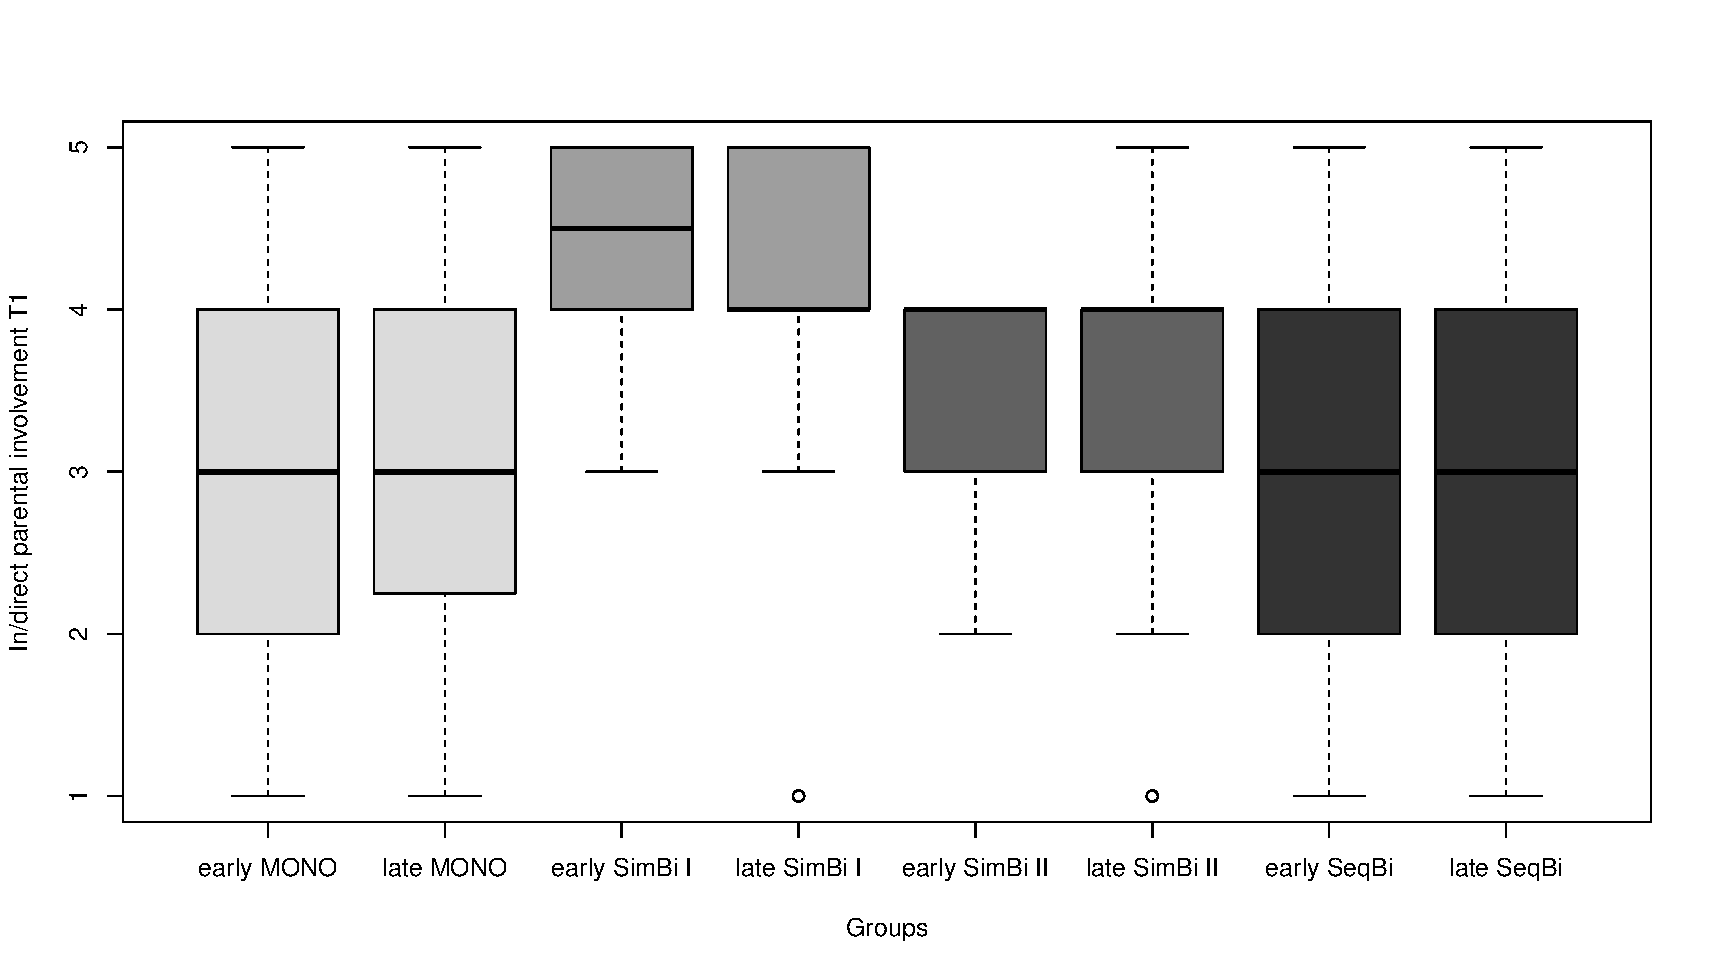
\includegraphics[width=\textwidth]{figures/pfenningerfig1.pdf}
\caption{\label{fig:pfenninger:1} In/direct parental involvement by AO and language group at Time 1}
\end{figure}

\begin{figure}%originally as fig 11 in the text, but it is actuallly the second image
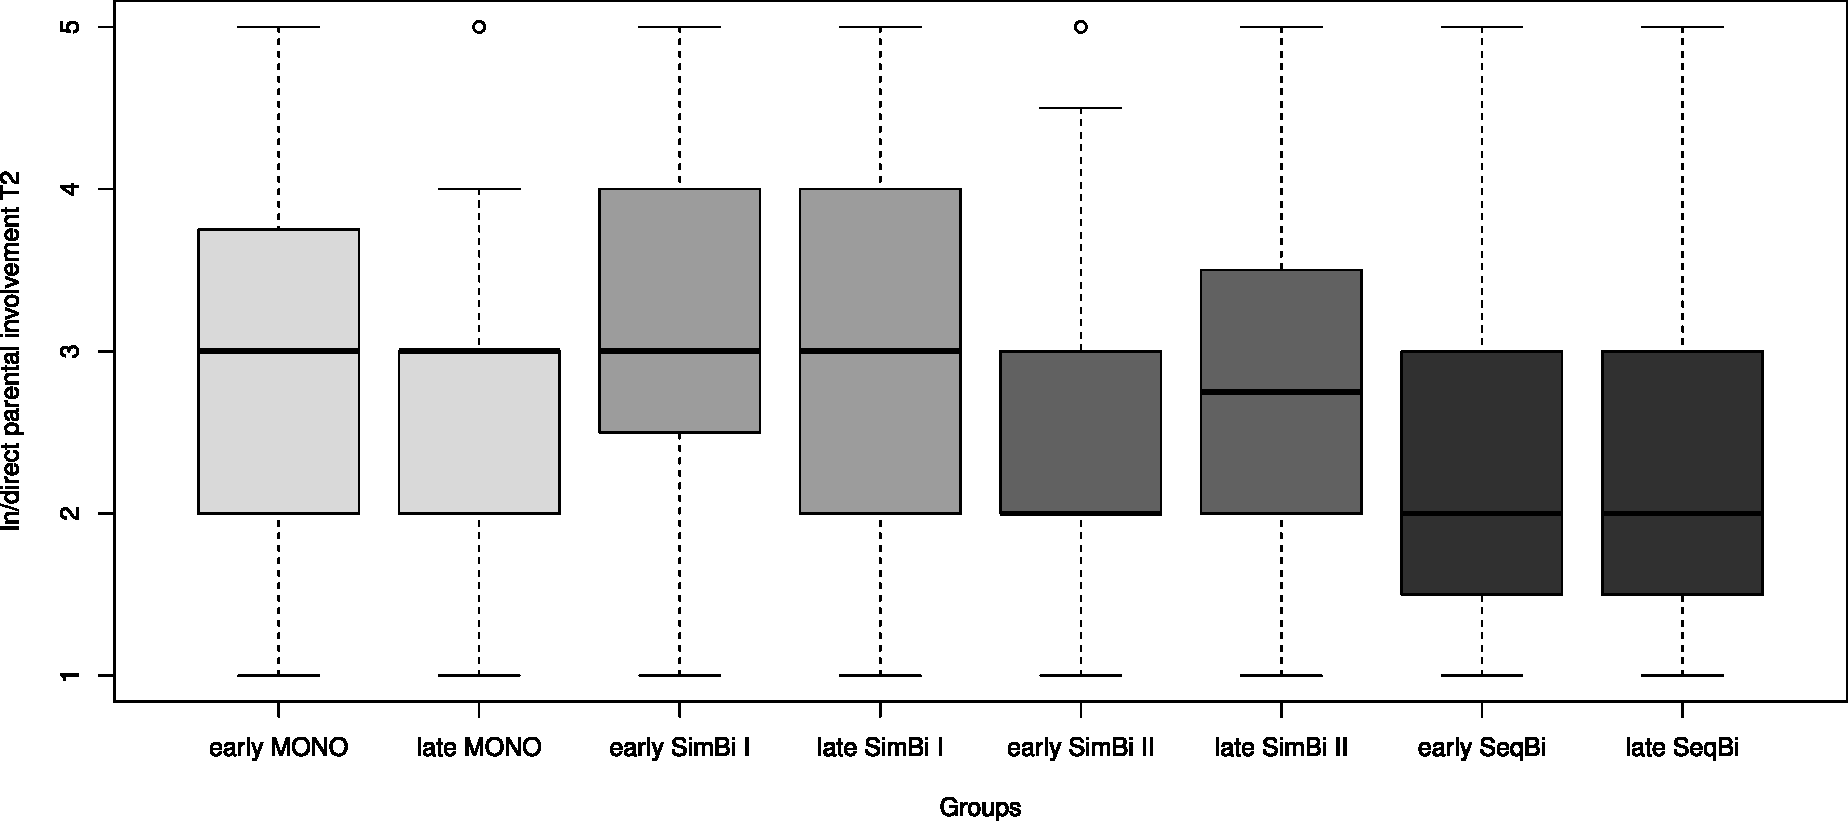
\includegraphics[width=\textwidth]{figures/PfenningerFigure2.pdf}
\caption{\label{fig:pfenninger:2} In/direct parental involvement by AO and language group at Time 2}
\end{figure}

Family circumstance – as measured by number of books/e-books in the household, frequency with which the parents read with/to their children and in/direct parental involvement in child’s study and education – predicted between 50\% and 75\% of the EFL measures, irrespective of AO and biological age of the participants (see Tables \ref{tab:pfenninger:14}--\ref{tab:pfenninger:19} in Appendix B). While each language group was similarly affected by home context, there were significant interactions between biliteracy and family circumstance across all FL measures as the SIMBI I group received substantially more parental support than the other groups (see also \citealt{PfenningerSingleton2019}).

Turning to simultaneous vs. sequential bilinguals, the findings revealed significant differences between them at the beginning and at the end of secondary school, with simultaneous bilinguals clearly outperforming monolinguals and sequential bilinguals (see e.g. Figures \ref{fig:pfenninger:3}--\ref{fig:pfenninger:4} for receptive vocabulary). However, when the samples were controlled for biliteracy, these differences had vanished by Time 2 (see Figures \ref{fig:pfenninger:5}--\ref{fig:pfenninger:6} ).% originally figures numbered as: 1, 2; and 3, 4.

\begin{figure} % originally figure 1
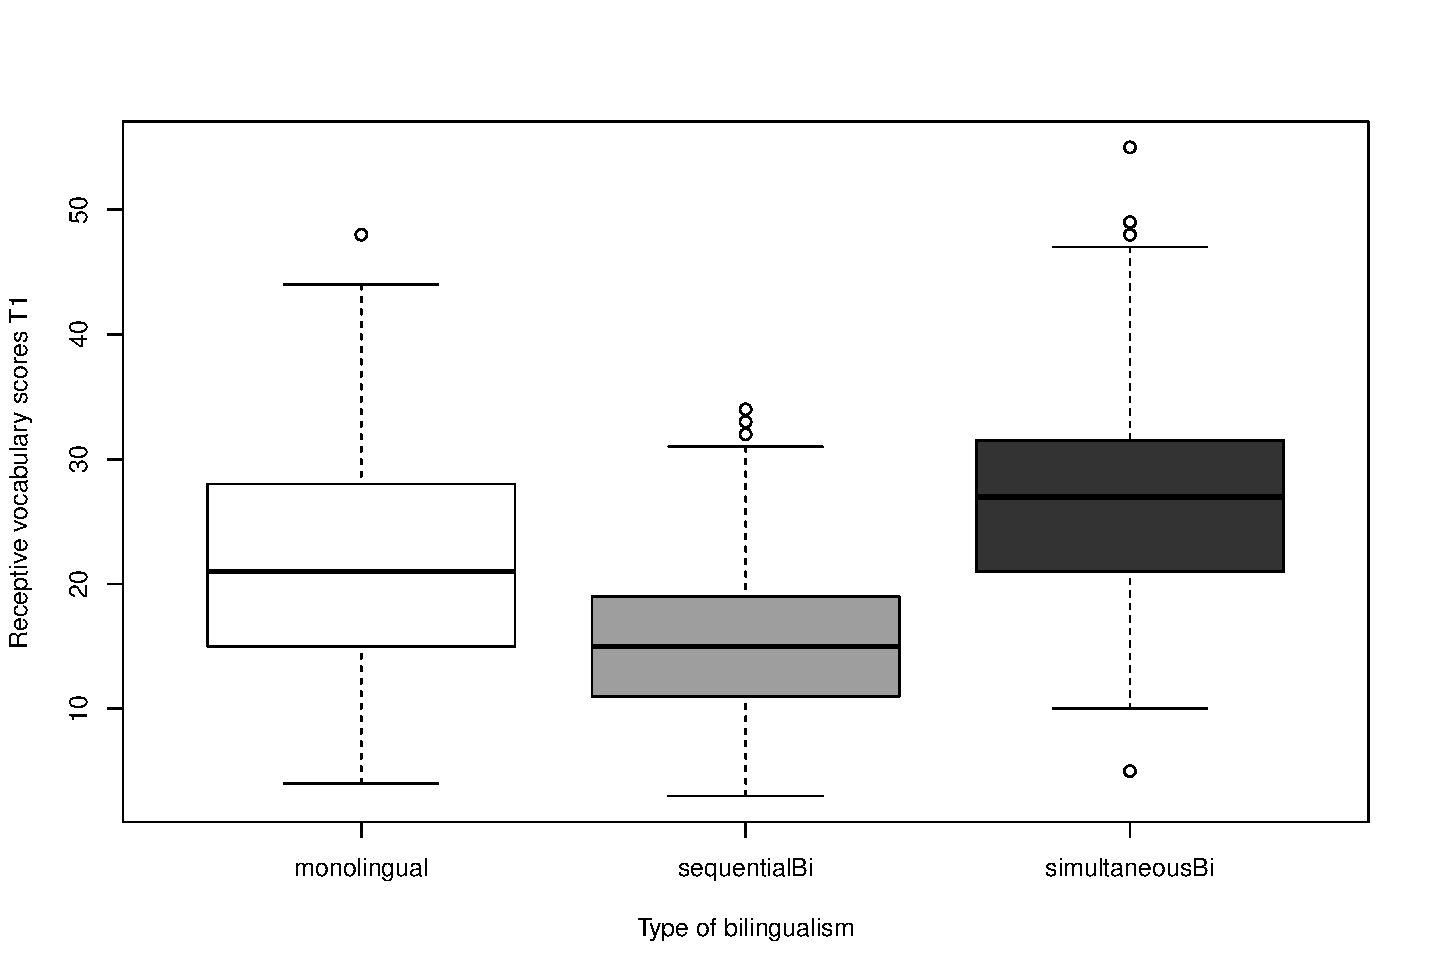
\includegraphics[width=.75\textwidth]{figures/PfenningerFigure3.pdf}
\caption{\label{fig:pfenninger:3}Receptive vocabulary by type of bilingualism at Time 1}
\end{figure}

\begin{figure} % originally figure 2
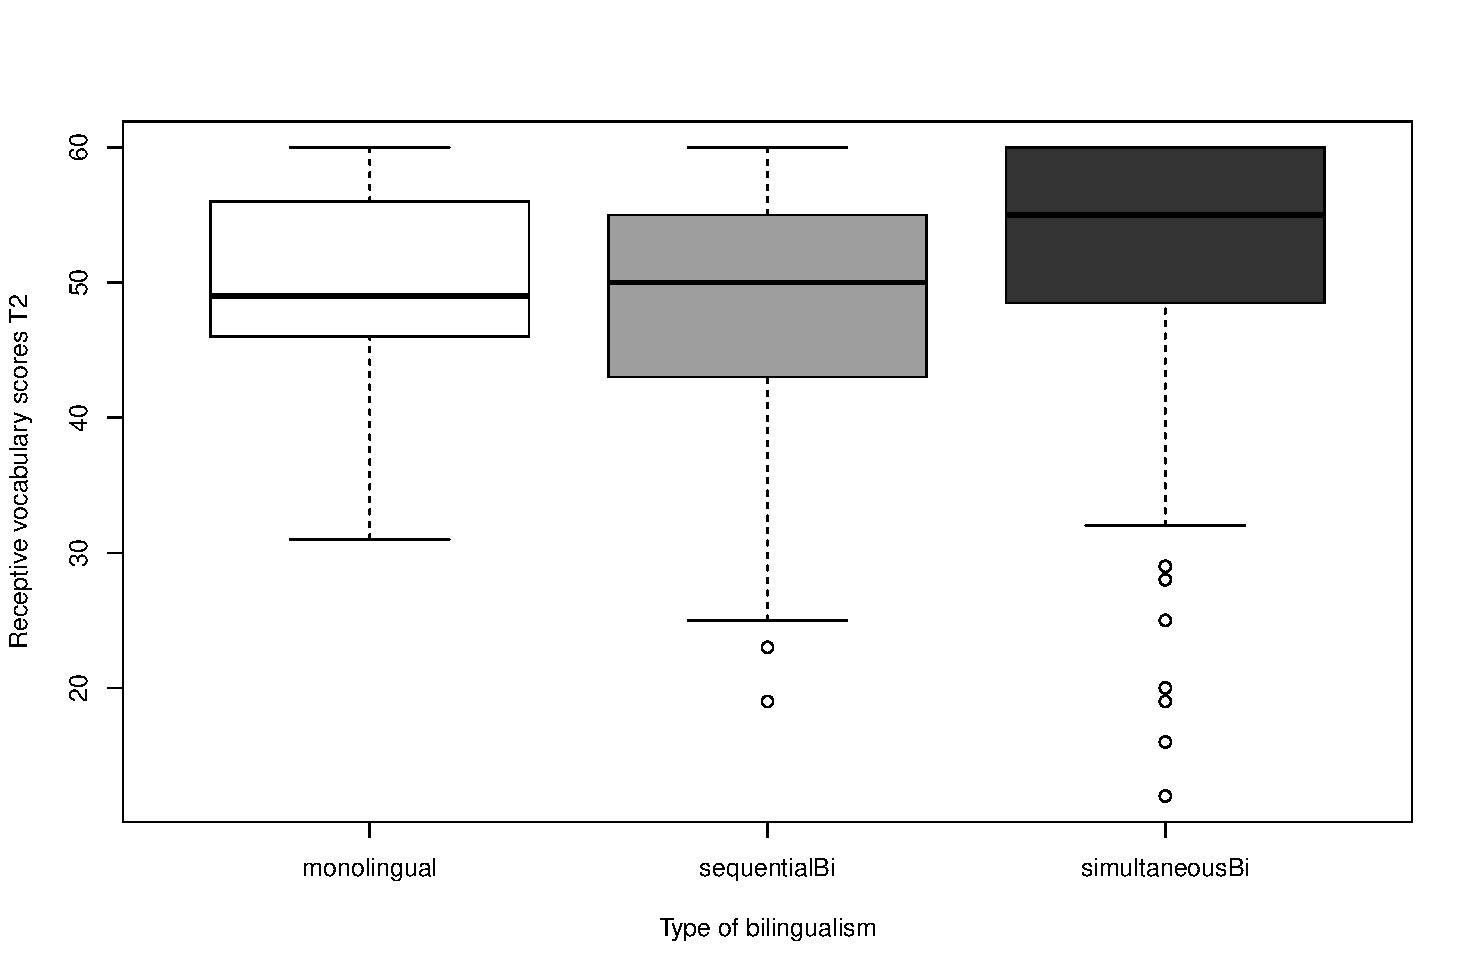
\includegraphics[width=.75\textwidth]{figures/PfenningerFigure4.pdf}
\caption{\label{fig:pfenninger:4}Receptive vocabulary by type of bilingualism at Time 2}
\end{figure}

\begin{figure} % originally figure 3
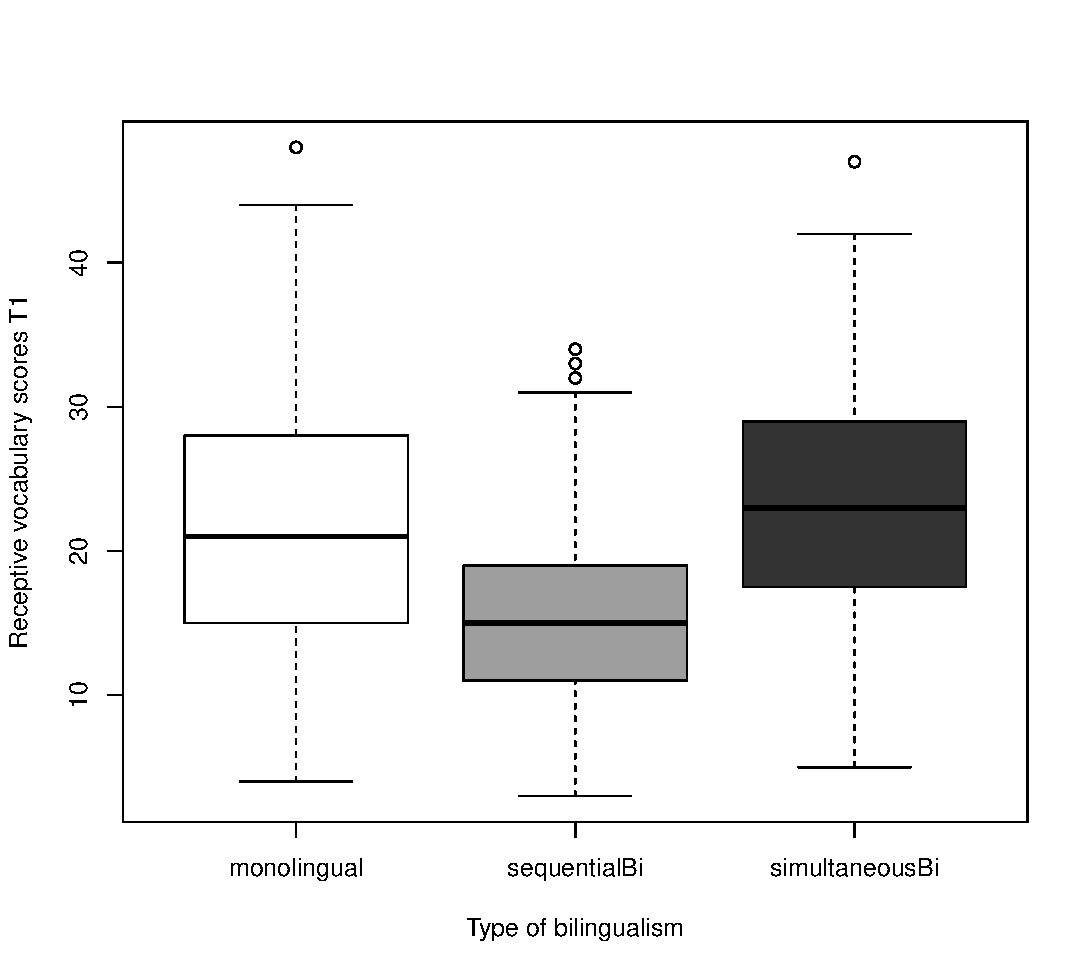
\includegraphics[width=.75\textwidth]{figures/PfenningerFigure5.pdf}
\caption{\label{fig:pfenninger:5}Receptive vocabulary by type of bilingualism (w/o biliterates) at Time 1}
\end{figure}

\begin{figure} % originally figure 4
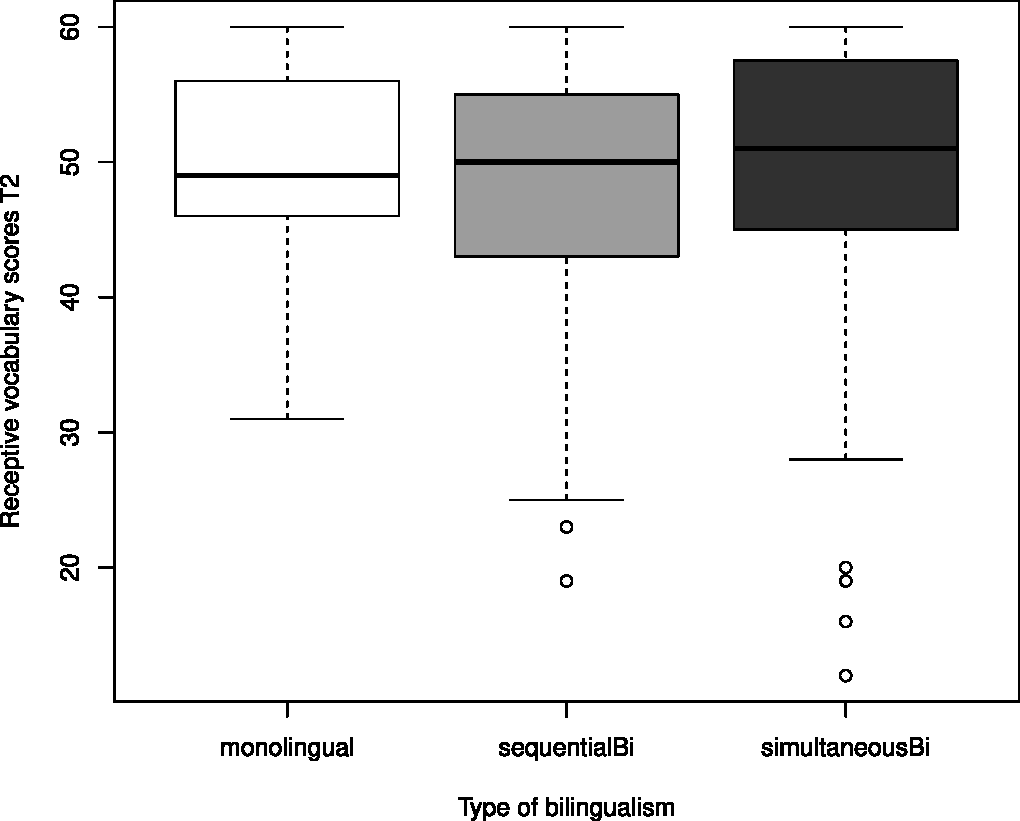
\includegraphics[width=.75\textwidth]{figures/PfenningerFigure6.pdf}
\caption{\label{fig:pfenninger:6} Receptive vocabulary by type of bilingualism (w/o biliterates) at Time 2}
\end{figure}

\subsection{RQ2: {How} {do} {literacy} {skills} {in} {the} {L1(s)} {affect} {literacy} {development} {in} {EFL?}}

% Tables \ref{tab:pfenninger:10} and \ref{tab:pfenninger:11} show the predictive power of the influence of German literacy on English literacy (for descriptive statistics see Tables \ref{tab:pfenninger:12}-\ref{tab:pfenninger:13} in Appendix B)\todo{check table nrs}.

\begin{table}
\caption{\label{tab:pfenninger:10}Impact of Standard German writing ability on English writing ability at Time 1}
\begin{tabular}{lS[table-format=-1.3\pm1.3,parse-numbers=false]S[table-format=1.2]S[table-format=<1.3,table-space-text-post = ab]}
\lsptoprule
& {Estimate ± SE} & {$t$}  & {$p$}\\\midrule
Written content (English) & 0.22±0.03 & 6.56 & <.001**\\
Written organization (English) & 0.12±0.03 & 4.12 & <.001**\\
Written lexical richness (English) & 0.08±0.03 & 2.51 & .008*\\
Written fluency (English) & 6.01±1.01 & 5.39 & <.001**\\
Written complexity (English) & 0.10±0.02 & 4.89 & <.001**\\
\lspbottomrule
\end{tabular}
\end{table}

\begin{table}
\caption{\label{tab:pfenninger:11}Impact of Standard German writing ability on English writing ability at Time 2. * $p<0.05$, ** $p<0.001$.}
\begin{tabular}{lS[table-format=-1.3\pm1.3,parse-numbers=false]S[table-format=1.2]S[table-format=<1.4,table-space-text-post = ab]}
\lsptoprule
& {Estimate ± SE} & {$t$}  & {$p$}\\\midrule
Written content (English) & 0.21±0.05 & 4.38 & <.001**\\
Written organization (English) & 0.38±0.07 & 5.49 & <.001**\\
Written lexical richness (English) & 0.16±0.04 & 3.71 & .0002**\\
Written fluency (English) & 0.16±0.07 & 2.23 & .034*\\
Written complexity (English) & 0.27±0.04 & 7.26 & <.001**\\
\lspbottomrule
\end{tabular}
\end{table}


L1 literacy skills were clearly positively related to L2 literacy skills in all groups, predicting written content, organization, lexical richness, fluency and complexity, as \figref{fig:pfenninger:7} and \figref{fig:pfenninger:8} illustrate for written fluency scores (see also \citealt{Pfenninger2014}).


\begin{figure}%fig 5 originally
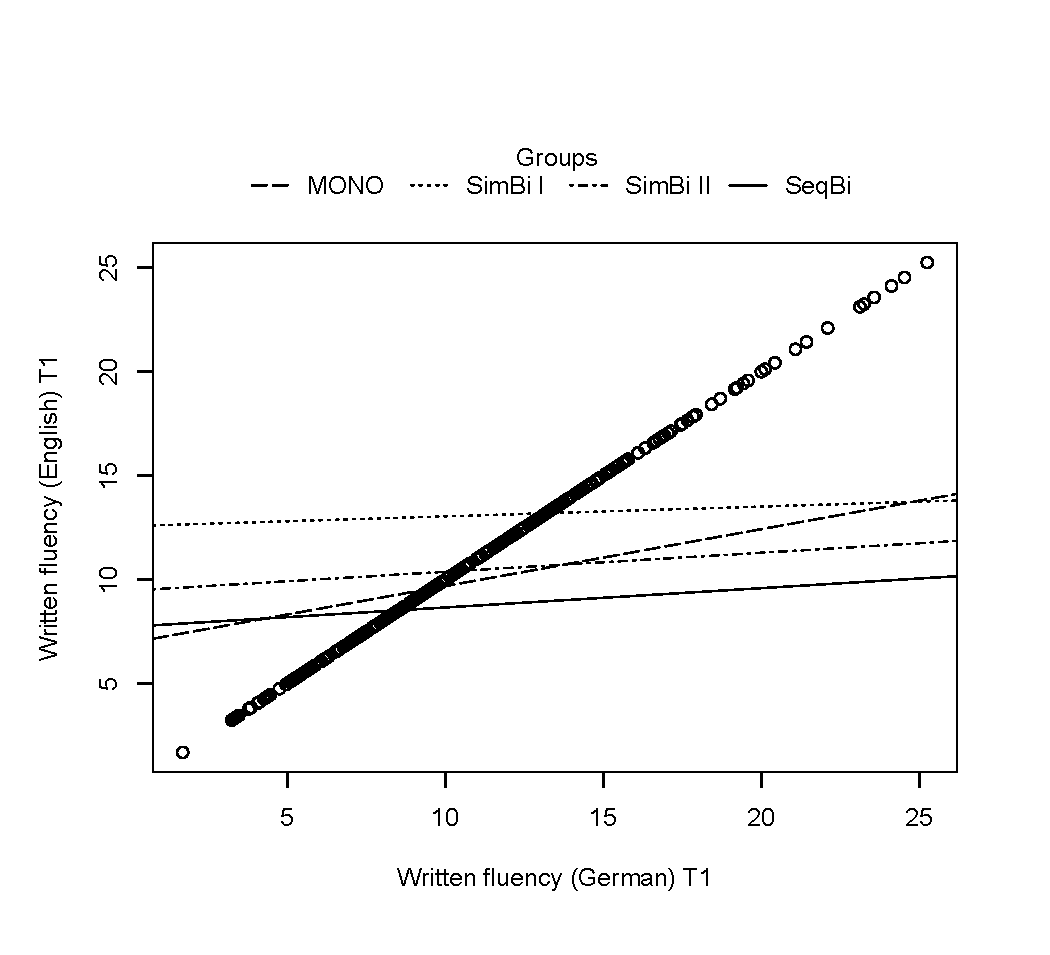
\includegraphics[height=.45\textheight]{figures/PfenningerFigure7.pdf}
\caption{\label{fig:pfenninger:7}Impact of written fluency (German) on language group at Time 1}
\end{figure}

\begin{figure}%fig 6 originally
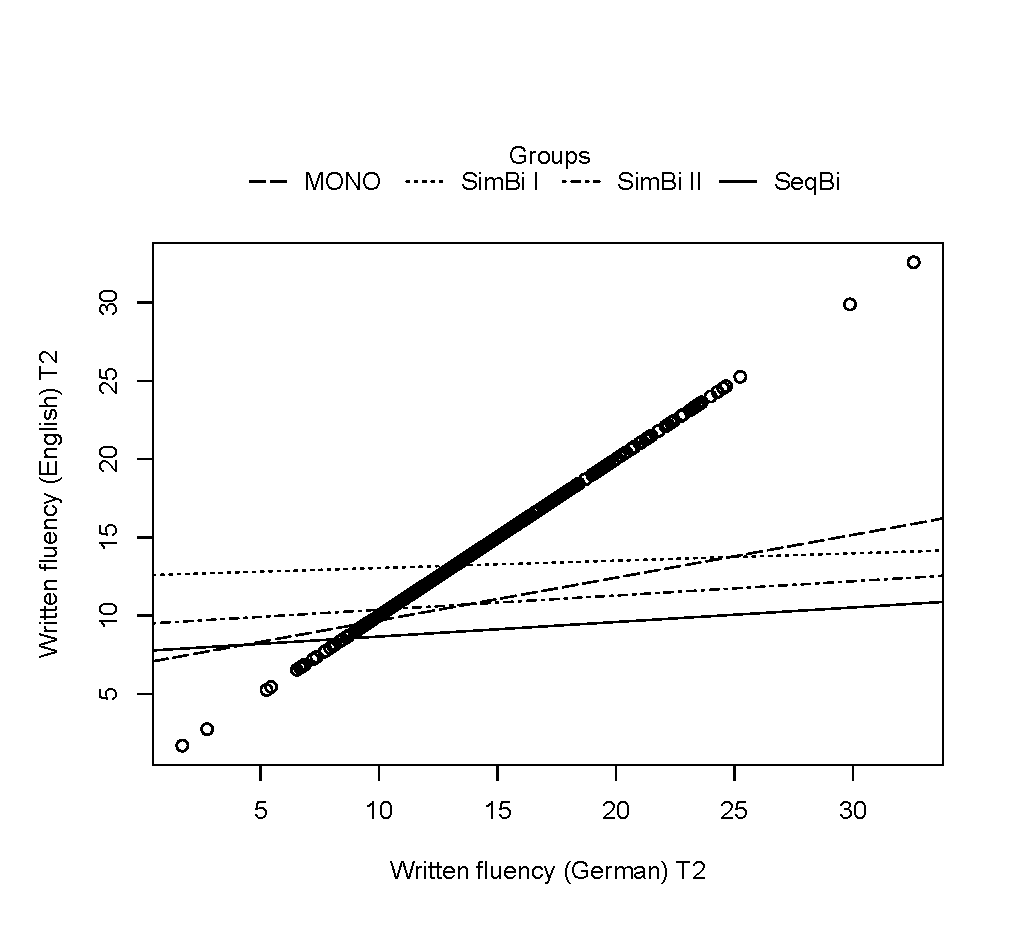
\includegraphics[height=.45\textheight]{figures/PfenningerFigure8.pdf}
\caption{\label{fig:pfenninger:8} Impact of written fluency (German) on language group at Time 2}
\end{figure}


The association between German literacy and English literacy is important inasmuch as the mixed models yielded statistically significant differences across language groups as well as across AO groups with respect to German writing performance: on the one hand, late starters consistently outperformed early starters in each language group at the beginning of secondary school; on the other hand, there were significant interactions between language group and German literacy skills at Time 1, as the sequential bilinguals (SEQBI group) had significantly lower scores across all skills tested (see \figref{fig:pfenninger:9}--\ref{fig:pfenninger:10} for written fluency and written content respectively). At the end of secondary school, these differences had disappeared (see e.g. \figref{fig:pfenninger:11} for written fluency and Tables \ref{tab:pfenninger:12}--\ref{tab:pfenninger:13} in Appendix B).%\todo{check table nrs}


\begin{figure}%fig 7
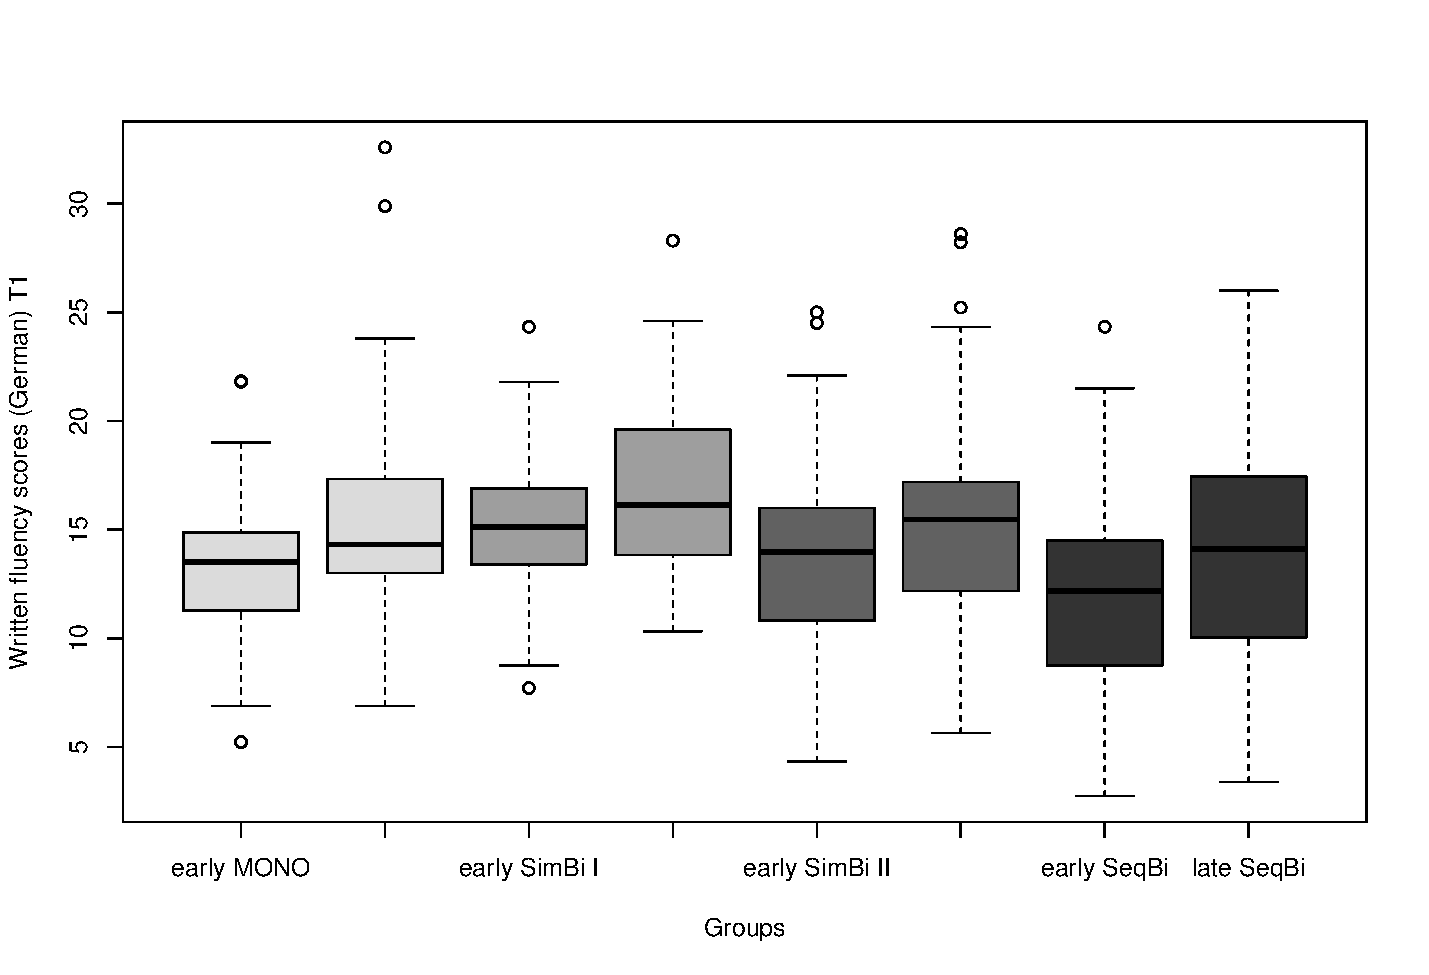
\includegraphics[height=.45\textheight]{figures/PfenningerFigure9.pdf}
 \caption{\label{fig:pfenninger:9}Written fluency (German) by AO and language group at Time 1}
\end{figure}


\begin{figure}% fig 8
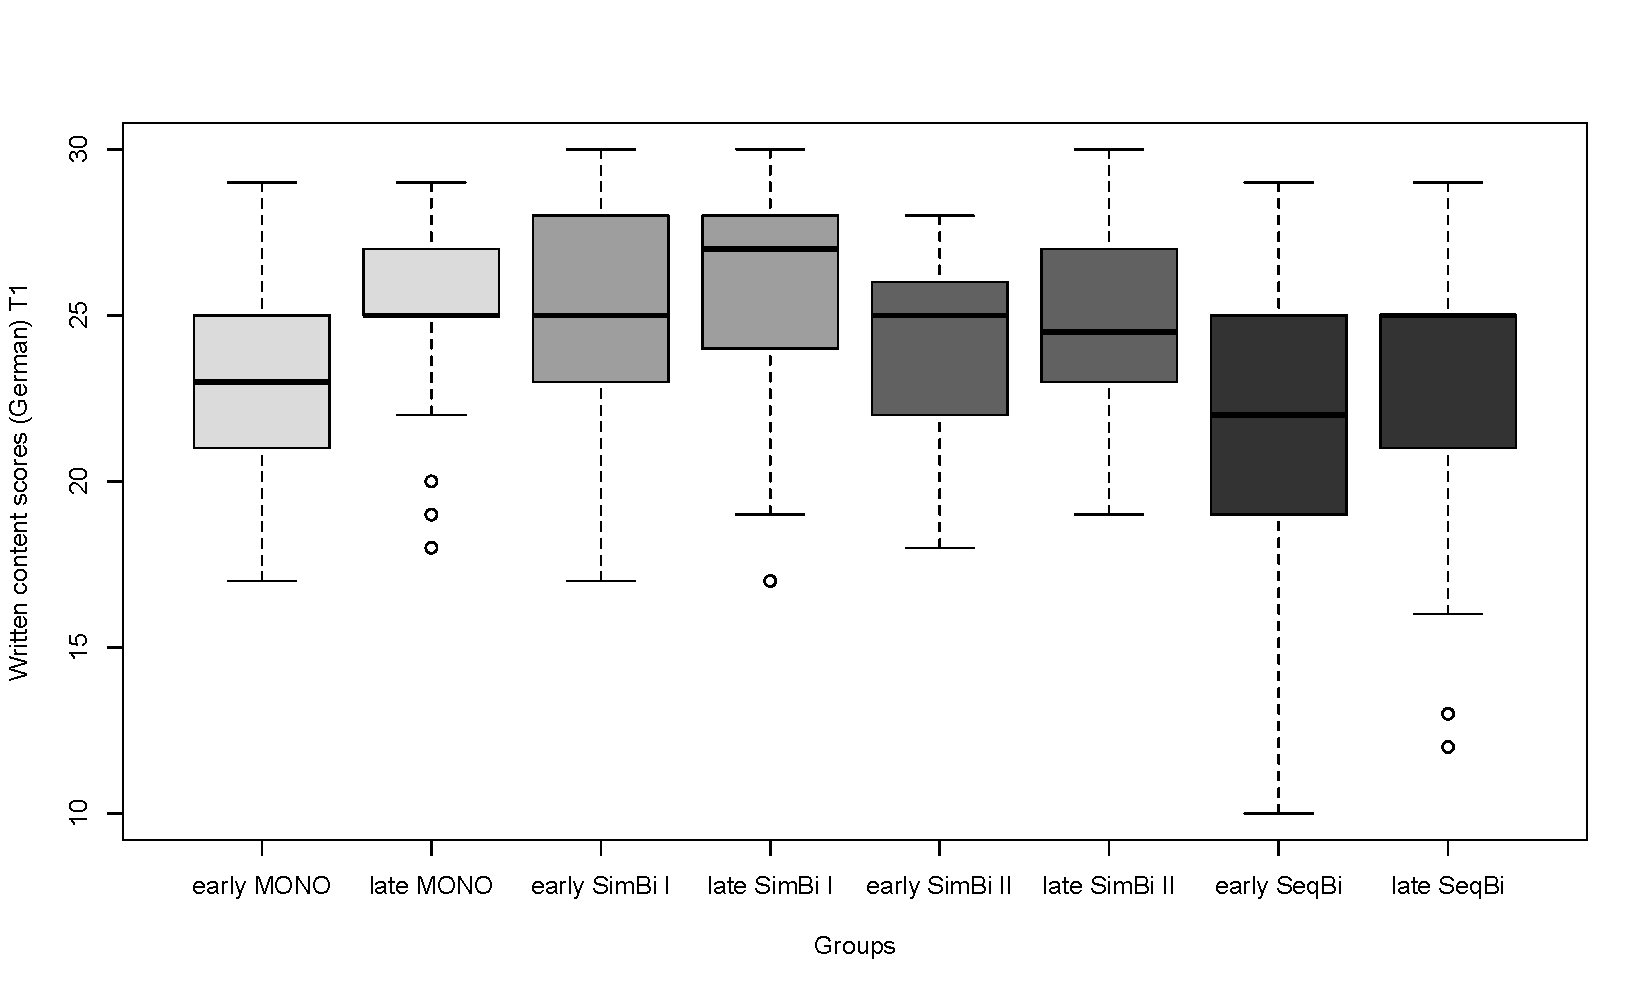
\includegraphics[width=\textwidth]{figures/PfenningerFigure10.pdf}
\caption{\label{fig:pfenninger:10} Written content (German) by AO and language group at Time 1}
\end{figure}


\begin{figure}%fig 9
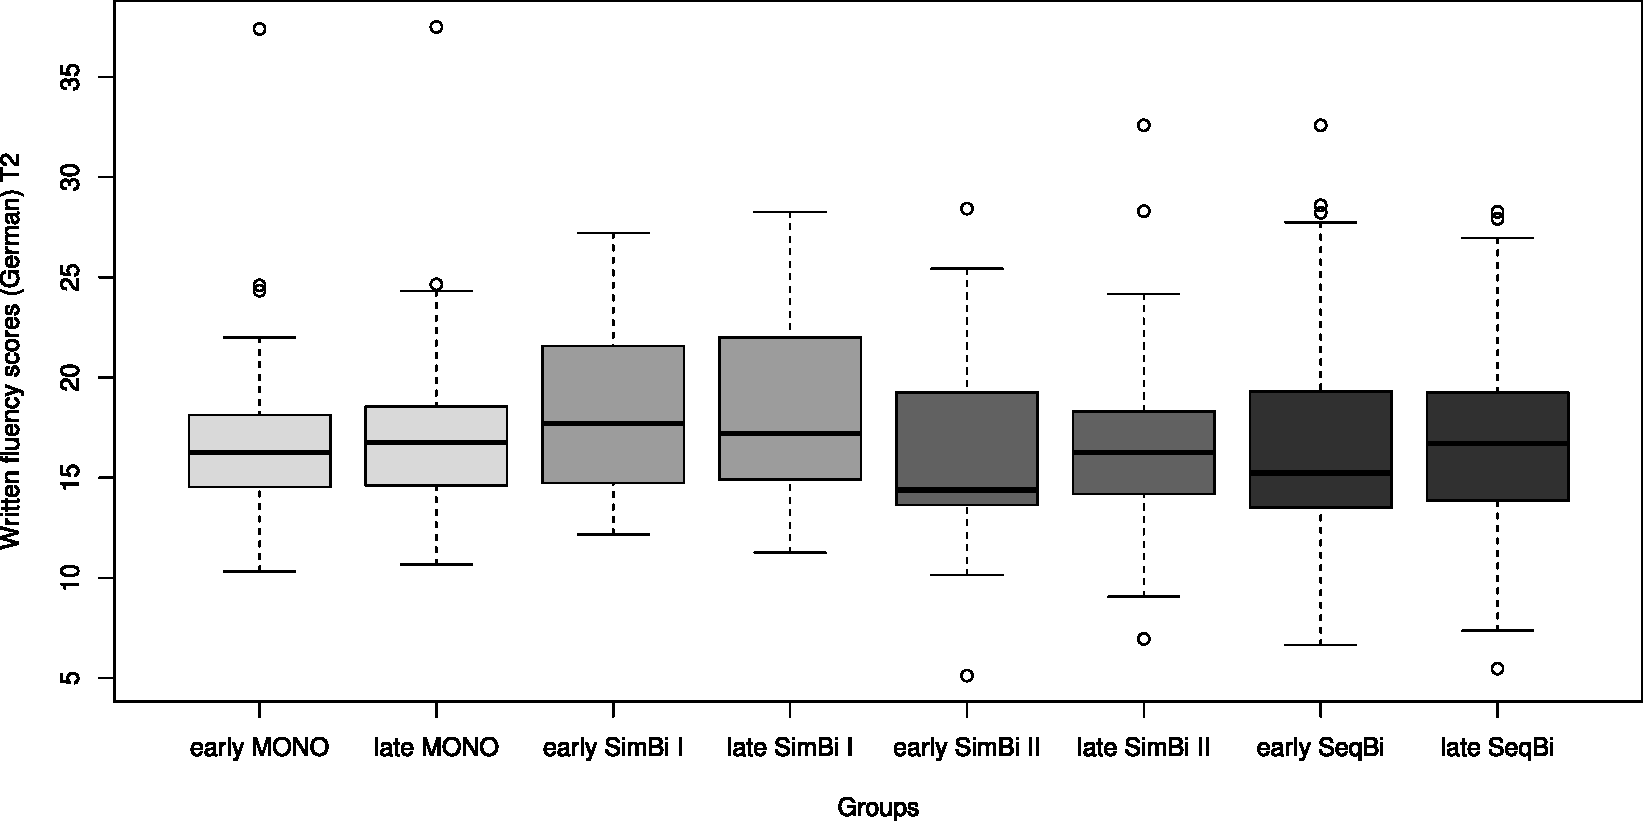
\includegraphics[width=\textwidth]{figures/PfenningerFigure11.pdf}
\caption{\label{fig:pfenninger:11} Written fluency (German) by AO and language group at Time 2}
\end{figure}

\section{Discussion}

On the one hand, the results of this study shed light on the susceptibility of different learner groups to an earlier vs. later starting age in FL learning and the importance of literacy skills in the L1(s); on the other hand, they revealed the mitigating influence of the hybridity of experiences of bilinguals on AO effects. While three out of the four groups tested (the monolinguals, simultaneous bilinguals (SIMBI II), and sequential bilinguals) displayed AO effects that are typical of monolinguals in school contexts – unstable temporary benefits of an earlier start – the simultaneous bilingual-biliterates (SIMBI I group) showed a pattern that is more reminiscent of naturalistic settings: the earlier the AO, the better the FL outcome in the long run.

A close analysis of the strength of the individual predictors as well as the interaction between them showed that this might be due to the fact that the SIMBI I participants were biliterate on top of being bilingual. Growing up bilingual endowed them with different preliteracy knowledge than monolingual children, as they had to acquire concepts of sound, word, and the function of print in their different languages before they could read \citep{Bialystok2007}. \citet{Bialystok2007} also suggests that the early experience of knowing two languages influences the acquisition of literacy; she hypothesizes that one avenue of that influence may be through the type of oral competence established by these children.

However, while bilingualism per se did not have an effect on the EFL outcome, unless it was coupled with a supportive learning environment, biliteracy impacted on most of the EFL measures. Before the SIMBI I group began primary school, they showed emergent literacy skills (developmental precursors to literacy) in two languages, both of which were later consolidated. In fact, these participants displayed very strong German literacy skills at Time 1, outperforming the other groups with respect to content, organization, fluency, complexity and accuracy of written output. Considering the high impact of German literacy skills on English literacy skills, it is perhaps not surprising that the SIMBI I had a temporary advantage in this realm. They might also benefit from heightened metalinguistic insights, which results from exposure to literacy in two languages (\citealt{Sanz2000, Bialystok2007}).

Finally, it is noteworthy that the SIMBI I group also received support from parents who encouraged biliteracy, owned a lot of books and had a habit of reading regularly to their children. Although emergent literacy skills could not be measured before primary school, we know that the parents of the SIMBI I students encouraged bilingual literacy skills from an early age on, i.e. they valued literacy skills in the home language highly. The SIMBI I students (both early and late starters) thus received more literacy support in their L1s than the early and late SEQBI participants. In the light of studies in Spain described in the literature review (e.g. \citealt{Sanz2008}), where bilinguals are always biliterate and no “earlier is better” effect could be observed for biliterate bilinguals, the main distinguishing factor may be parental support rather than biliteracy in this study.

This leads us to the question as to why the early starters in the other two bilingual groups (SIMBI II and SEQBI) could not benefit more from their earlier start, i.e. why they show similar AO effects as the monolingual students. One potential reason for this is that they were not biliterate; the SEQBI participants, for instance, had virtually no literacy skills in their home language at the first data collection time. Before they had begun primary school, they showed emergent literacy skills (developmental precursors to literacy) in their L1 (not German) according to their parents, but this effort was later abandoned. While they received the same amount of literacy support in German as the SIMBI groups, there was a common belief among their parents that native language use at home interferes with the acquisition of L2 learning at school.

The SEQBI group also had poorer L2 (German) literacy skills than the other groups at the beginning of secondary school, arguably due to slowly developing literacy skills throughout primary school: when they began L3 English instruction in second grade, they were only marginally bilingual and were typically exposed to the oral and written forms of their L2 (German) simultaneously (see also the results in \citealt{SánchezBardel2017}). Referring to a number of other authors (e.g. \citealt{Collier1987, Cummins1991, AugustHakuta1997}), \citet{Bialystok2007} points out that children who acquire language literacy in school in spite of having a weak oral command of that language typically achieve lower levels of reading competence than their peers and require between four and seven years to reach grade-level standards in academic and literacy achievement. \citet[22]{Bialystok2007} adds that “[m]ore important, however, is that the social and educational background of these children may compromise their ability to acquire literacy, irrespective of language proficiency”.

It needs to be emphasized, however, that there were no more differences between early and late monolinguals, simultaneous bilinguals, and sequential bilinguals at the end of mandatory school time. The fact that the early starters’ lag in German literacy skills – as well as the differences between simultaneous and sequential bilinguals – were of temporary nature should provide reassurance to educators and parents that (1) students’ L1 literacy skills will not be sacrificed by an early EFL program and (2) early bilingualism does not jeopardize either the development of literacy skills in the community language or the acquisition of an additional L2 – quite to the contrary!\\

%section 6
\section{Conclusions and implications}
\label{sec:pfenninger:6}

Of prime interest in this study was how an earlier vs. later AO influences the EFL outcomes of different learner groups (monolinguals vs. bilinguals, simultaneous vs. sequential bilinguals and bilinguals vs. biliterates). The results of a longitudinal analysis with 636 secondary school students revealed that an earlier AO is only beneficial for one specific learner group across a range of productive and receptive, oral and written FL measures: simultaneous bilinguals who are biliterate and receive substantial parental support (in the short and the long-run), as opposed to monolinguals and non-biliterate bilinguals (simultaneous or sequential), who do not benefit from an earlier AO in the long run.

Besides these differential AO effects, the results also revealed that sociolinguistic context in which languages are highly valued may also have positive consequences with respect to the bilingual advantage. Quality in the home environment seems to be important regardless of differences in AO or biological age (see also \citealt{PfenningerSingleton2019}). The beneficial effects of parental sensitivity maps onto the bilingualism literature quite well. For instance, family circumstances in which bilingualism is valued provide children with the opportunities to use and switch between two languages, which in turn could enhance their executive functions (see \citealt{GoriotEtAl2016}). The lack of difference in additional language learning between monolingual and bilingual students is informative, confirming that we cannot ignore the fact that many factors affect the language acquisition process, and bilingualism is an important but not exclusive influence (see e.g. \citealt{Cenoz2009}). Also, the fact that there are no differences between simultaneous vs. sequential bilinguals when biliteracy is controlled for highlights the heterogeneity of bilingual populations and the importance of distinguishing between different types of bilinguals.

The results from this study also have important educational implications in light of the increasing number of multilingual students (e.g. children with an immigrant background), who, in the early primary grades, have to learn and become literate in two languages other than the one first learned at home. While the observation that almost all subskills that form an integral part of the skill of L2 writing correlate with L1 writing ability is not new, one of the remarkable outcomes of this study involves the lag in the development of German writing ability among early starters in each language group. Thus, L1 and L2 educators and policy makers should understand that mastery of literacy skills in the elementary school years is important for students attempting to learn a FL several years later, as already discussed in \citet{Pfenninger2014}.

The importance of L1 literacy skills calls for research that identifies and evaluates best practices regarding support of language and literacy development for multilingual children. Parents, teachers, and policy-makers should be made aware of the benefits of bilingualism, and the consequences of their appreciation of different L1s for children’s cognition. According to \citet{GoldenbergEtAl2006}, instructional enhancements are necessary to support sequential bilinguals’ language and literacy development, especially when instruction is conducted only in the language of the community. This means that teachers need to be better trained to work with and enhance language and literacy among dual language learners. There is also a dearth of intervention studies focusing on promoting multilingual language and literacy development in young learners who are not yet proficient in the language of the target culture (here German) (see \citealt{AugustShanahan2006}).

Finally, I note some limitations of this study. At the beginning of primary school, the sequential bilinguals were learning literacy skills in their weak language (German) at the same time as they were learning to read in their strong language (L1), which means that the transfer of skills from the dominant language might have facilitated literacy in the weaker language, obscuring any effect that bilingualism per se might have imparted (see \citealt{Bialystok2007}). In future studies it would be fruitful to add balance to the equation and analyze if more balanced use and a more balanced level of proficiency of two languages within the bilingual groups has significant effects~on the L3 learning outcome. \citet{YowLi2015}, for instance, found a significant effect of the latent variable balanced bilingualism (balanced usage and proficiency in two languages) on certain components of executive functioning – \textit{in} \textit{addition} to effects of the impact of age of L2 acquisition. In a next step it would also be interesting to analyze the same variables in a comparable socio-educational context that involves typologically different languages. In the present study, language typology is not a variable under analysis. I made sure, however, that the participants in the three bilingual groups came from the same L1 backgrounds (Spanish, Portuguese, Croatian, Serbian, Albanian, Arabic, or Italian) by controlling the number of L1s in each group. None of these languages were part of the school curriculum. What is more, we find the same number and types of language pairs (e.g. German-Albanian, German-Serbian) in each bilingual group. Nevertheless, in considering these arguments, the reader should bear in mind that the relationship among the languages involved might also account for differences in the results of research on the effects of bi/literacy on L3 learning.

\appendixsection{Appendix A}

Time 1:


Receptive vocabulary (Biliteracy:InB\_Parents β=-1.41±0.45, t=-3.10),\\
 lexical richness (Bilingualism:AttitudesParents β=-0.21±0.09, t=-2.28, Biliteracy:InB\_Parents (β=-0.25±0.07, t=-3.63),\\
 written fluency (Bilingualism:Books β=-0.95±0.43, t=-2.20, Bilingualism:DirB β=-1.43±0.32, t=-4.49),\\
 written complexity (Bilingualism:AttitudesParents β=-0.07±0.03, t=-2.30, Biliteracy:InB\_Parents β=-0.06±0.02, t=-2.76, Biliteracy:AttitudesParents β=-0.11±0.05, t=-2.52),\\
 written accuracy (Biliteracy:AttitudesParents β=0.15±0.09, t=2.01),\\
 oral lexical richness (Bilingualism:DirB β=-0.25±0.13, t=-2.03),\\
 oral fluency (Bilingualism:DirB β=-2.58±1.25, t=-2.07, Biliteracy:Score1.DirB β=-2.82±2.01, t=1.41),\\
 oral complexity (Biliteracy:InB\_Parents β=-0.10±0.03, t=-3.03, Biliteracy:AttitudesParents β=-0.16±0.06, t=-2.46),\\
 oral accuracy (Bilingualism:Books β=0.42±0.20, t=2.10, Biliteracy:AttitudesParents β =0.73±0.22, t=3.13),\\
 and grammaticality judgments (Bilingualism:DirB β=-0.77±0.36, t=-2.14);


Time 2:


Listening comprehension (Bilingualism:Books β=-0.76±0.42, t=-1.82, Bilingualism:DirB β=-0.84±0.27, t=-3.12),\\
 productive vocabulary (Bilingualism:Books β=--2.55±0.88, t=-2.91, Bilingualism:DirB β=-1.18±0.54, t=-2.17, Biliteracy:Score.Books β=-3.32±1.39, t=-2.38, Biliteracy:Score.IndB\_Parents β=-1.74±0.48, t=-3.65),\\
 receptive vocabulary (Bilingualism:DirB β=-1.22±0.63, t=-1.95, Biliteracy:IndB\_Parents β=-1.42±0.53, t=-2.69, Biliteracy:Score2.DirB β=1.21±0.70, t=1.71),\\
 written lexical richness (Bilingualism:AttitudesParents β=-0.18±0.08, t=-2.19, Biliteracy:Score2.DirB β=0.16±0.08, t=1.91),\\
 written fluency (Bilingualism: Books β=-1.89±0.47, t=-4.03),\\
 written complexity (Bilingualism:AttitudesParents β=-0.09±0.04, t=-2.49, Biliteracy:InB\_Parents β=-0.08±0.03, t=-2.42, Biliteracy:Score2.DirB β=-0.10±0.04, t=-2.57),\\
 written accuracy (Bilingualism:Books β=0.17±0.06, t=2.68, Bilingualism:DirB β=0.13±0.04, t=3.08, Biliteracy:Score2.DirB β=-0.14±0.06, t=-2.94),\\
 oral lexical richness (Bilingualism: DirB β=-0.31±0.10, t=-3.28, Biliteracy:InB\_Parents β=-0.24±0.08, t=-2.87),\\
 oral accuracy (Bilingualism:InB\_Parents β=0.39±0.14, t=2.81, Bilingualism:DirB β=0.26±0.11, t=2.41, Biliteracy:Score.Books β=1.23±0.26, t=4.64),\\
 oral fluency (Biliteracy:InB\_Parents β=-1.73±0.86, t=-2.01),\\
 oral complexity (Biliteracy:Score.AttitudesParents β=0.06±0.04, t=1.32),\\
 and grammaticality judgments (Bilingualism:AttitudesParents β=-1.13±0.31, t=-3.62, Biliteracy:Score2.DirB β=-0.85±0.32, t=-2.68).


\appendixsection{Appendix B}

\begin{sidewaystable}
\caption{Descriptive statistics (means and standard deviations) for German literacy}
\begin{subtable}[t]{\linewidth}
\caption{\label{tab:pfenninger:12}At Time 1}
{\scriptsize
\begin{tabular}{l *{8}{S[table-format=2.2]@{~}S[table-format=2.2,input-symbols={( )}]}}
\lsptoprule
 & \multicolumn{4}{c}{\textsc{Mono}} & \multicolumn{4}{c}{\textsc{SimBi1}}  & \multicolumn{4}{c}{\textsc{SimBi2}}  & \multicolumn{4}{c}{\textsc{SeqBi}}  \\
   \cmidrule(lr){2-5}\cmidrule(lr){6-9}\cmidrule(lr){10-13}\cmidrule(lr){14-17}
 & \multicolumn{2}{c}{\textsc{ECL}\textsubscript{1}}  &  \multicolumn{2}{c}{\textsc{LCL}\textsubscript{1}}   & \multicolumn{2}{c}{\textsc{ECL}\textsubscript{1}}  & \multicolumn{2}{c}{\textsc{LCL}\textsubscript{1}}  & \multicolumn{2}{c}{\textsc{ECL}\textsubscript{1}} & \multicolumn{2}{c}{\textsc{LCL}\textsubscript{1}}  & \multicolumn{2}{c}{\textsc{ECL}\textsubscript{1}}  & \multicolumn{2}{c}{\textsc{LCL}\textsubscript{1}} \\
 & \multicolumn{2}{c}{$n=100$} & \multicolumn{2}{c}{$n=100$} & \multicolumn{2}{c}{$n=73$} & \multicolumn{2}{c}{$n=71$} & \multicolumn{2}{c}{$n=57$} & \multicolumn{2}{c}{$n=50$} & \multicolumn{2}{c}{$n=95$} & \multicolumn{2}{c}{$n=90$}\\
\midrule
Written content (German)          &  23.17 & (2.77) &  24.65 & (2.16) &  24.82 & (3.43) &  25.93 & (3.10) &  23.63 & (2.68) &  24.48 & (2.57) &  21.27 & (3.82) &  22.82 & (4.52)\\
Written organization (German)     &  13.98 & (2.97) &  15.96 & (2.72) &  14.08 & (2.78) &  14.75 & (3.24) &  14.30 & (3.34) &  16.34 & (2.82) &  14.55 & (3.36) &  15.77 & (2.63)\\
Written lexical richness (German) &   7.24 & (1.28) &   7.90 & (1.30) &   7.30 & (1.53) &   7.92 & (1.38) &   7.54 & (1.33) &   8.24 & (1.19) &   7.31 & (1.58) &   7.72 & (1.32)\\
Written fluency (German)          &  13.08 & (3.23) &  15.20 & (4.17) &  15.49 & (3.17) &  16.83 & (4.00) &  13.47 & (4.26) &  15.56 & (4.97) &  11.58 & (4.26) &  13.72 & (5.41)\\
Written complexity (English)      &   1.60 & (0.57) &   1.89 & (0.67) &   1.83 & (0.65) &   2.01 & (0.66) &   1.76 & (0.69) &   1.86 & (0.74) &   1.62 & (0.53) &   1.75 & (0.60)\\
\lspbottomrule
\end{tabular}}
\end{subtable}
\vskip2\baselineskip
\begin{subtable}[t]{\linewidth}
\caption{\label{tab:pfenninger:13}At Time 2}
{\scriptsize
\begin{tabular}{l *{8}{S[table-format=2.2]@{~}S[table-format=2.2,input-symbols={( )}]}}
\lsptoprule
 & \multicolumn{4}{c}{\textsc{Mono}} & \multicolumn{4}{c}{\textsc{SimBi1}}  & \multicolumn{4}{c}{\textsc{SimBi2}}  & \multicolumn{4}{c}{\textsc{SeqBi}}  \\
   \cmidrule(lr){2-5}\cmidrule(lr){6-9}\cmidrule(lr){10-13}\cmidrule(lr){14-17}
 & \multicolumn{2}{c}{\textsc{ECL}\textsubscript{1}}  &  \multicolumn{2}{c}{\textsc{LCL}\textsubscript{1}}   & \multicolumn{2}{c}{\textsc{ECL}\textsubscript{1}}  & \multicolumn{2}{c}{\textsc{LCL}\textsubscript{1}}  & \multicolumn{2}{c}{\textsc{ECL}\textsubscript{1}} & \multicolumn{2}{c}{\textsc{LCL}\textsubscript{1}}  & \multicolumn{2}{c}{\textsc{ECL}\textsubscript{1}}  & \multicolumn{2}{c}{\textsc{LCL}\textsubscript{1}} \\
 & \multicolumn{2}{c}{$n=100$} & \multicolumn{2}{c}{$n=100$} & \multicolumn{2}{c}{$n=73$} & \multicolumn{2}{c}{$n=71$} & \multicolumn{2}{c}{$n=57$} & \multicolumn{2}{c}{$n=50$} & \multicolumn{2}{c}{$n=95$} & \multicolumn{2}{c}{$n=90$}\\
\midrule
 Written content  (German)         & 28.71 & (1.43) &  28.57 & (1.87) &  28.07 & (2.30) &  28.48  & (2.01) &  28.18 & (2.26) &  28.12 & (2.26) & 28.32 & (1.75) &  28.68 & (1.80)\\
 Written organization (German)     &  18.39 & (2.72) &  18.33 & (1.67) &  18.44 & (1.50) &  18.06 & (1.76) &  18.75 & (1.47) &  18.54 & (1.33) &  18.38 & (1.58) &  18.17 & (1.76)\\
 Written lexical richness (German) &  9.02 & (0.88) &  9.03 & (0.76) &  9.11 & (0.73) &  9.19 & (0.79) & 9.20 & (0.93) &  9.26 & (0.93) &  8.63 & (1.41) &  9.13 & (0.80)\\
 Written fluency (German)          &  16.74 & (3.77) &  16.92 & (3.60) &  18.37 & (4.07) & 18.09 & (4.02) &  16.30 & (4.47) &  16.89 & (4.43) &  16.51 & (4.94) &  16.74 & (4.50)\\
 Written complexity (German)       &  2.11 & (0.47) &  2.19 & (0.51) &  2.14 & (0.58) &  2.01 & (0.43) &  2.20 & (0.52) &  2.15 & (0.41) &  2.09 & (0.51) &  2.08 & (0.40)\\
\lspbottomrule
\end{tabular}}
\end{subtable}
\end{sidewaystable}

\begin{table}
\caption{\label{tab:pfenninger:14}\label{tab:pfenninger:15}Multilevel regression analyses for environmental influences at Time 1 (fixed effect estimates for home variables). * $p <0.05$, ** $p<0.001$.}
\begin{tabular}{l S[table-format=-1.2\pm1.2,parse-numbers=false]SS}
\lsptoprule
& \multicolumn{3}{c}{Fixed effect: Books}\\\cmidrule{2-4}
 & {Estimate ± SE} & {$t$}  & {Main effect $p$}\\\midrule
Receptive vocabulary & 1.52\pm0.43 & 3.58 & .0003** \\
Written lexical richness & 0.15\pm0.06 & 2.34 & .018*  \\
Written fluency & 1.00\pm0.26 & 3.81 & .001**  \\
Written complexity & 0.03\pm0.02 & 1.49 & .129  \\
Written accuracy & -0.09\pm0.04 & -2.35 & .018*  \\
Oral lexical richness & 0.16\pm0.09 & 1.80 & .068\\
Oral fluency & 1.61\pm0.83 & 1.93 & .050*  \\
Oral complexity & 0.08\pm0.03 & 2.81 & .005**  \\
Oral accuracy & -0.48\pm0.13 & -3.75 & .001**  \\
GJT & -0.04\pm0.26 & -0.15 & .900 \\
\midrule
& \multicolumn{3}{c}{Fixed effect: Frequency of reading}\\\midrule
% % %  & {Estimate ± SE} & {$t$}  & {Main effect $p$}\\\midrule
Receptive vocabulary & 1.16\pm0.32 & 3.60 & .0002** \\
Written lexical richness & 0.08\pm0.05 & 1.72 & .087 \\
Written fluency & 1.15\pm0.20 & 5.62 & <.0001** \\
Written complexity & -0.00\pm0.02 & -0.26 & .790 \\
Written accuracy & -0.07\pm0.03 & -2.37 & .018* \\
Oral lexical richness & 0.22\pm0.08 & 2.70 & .024*\\
Oral fluency & 4.48\pm1.85 & 2.42 & .019* \\
Oral complexity & -0.02\pm0.02 & -1.09 & .276 \\
Oral accuracy & 0.01\pm0.10 & 0.09 & .908 \\
GJT & 0.56\pm0.26 & 2.14 & .050* \\
\lspbottomrule
\end{tabular}
\end{table}

\begin{table}
	\caption{\label{tab:pfenninger:16} Multilevel regression analyses for environmental influences at Time 1. Fixed effect estimates for home variable in/direct parental involvement. * $p <0.05$, ** $p<0.001$.}
	\begin{tabular}{l S[table-format=-1.2\pm1.2,parse-numbers=false]SS}
		\lsptoprule
		& \multicolumn{3}{c}{Fixed effect: In/direct parental involvement}\\\cmidrule{2-4}
		 & {Estimate ± SE} & {$t$}  & {Main effect $p$}\\\midrule
		Receptive vocabulary & 1.81\pm0.31 & 5.84 & <.0001** \\
		Written lexical richness & 0.13\pm0.06 & 2.24 & .037* \\
		Written fluency & 0.39\pm0.15 & 2.53 & .010*\\
		Written complexity & 0.13\pm0.04 & 3.12 & .001**\\
		Written accuracy & 0.01\pm0.03 & 0.39 & .702\\
		Oral lexical richness & -0.04\pm0.06 & -0.62 & .538\\
		Oral fluency & 0.57\pm0.60 & 0.94 & .956\\
		Oral complexity & 0.18\pm0.10 & -3.01 & .010*\\
		Oral accuracy & -0.69\pm0.21 & -3.31 & .004**\\
		GJT & 0.20\pm0.19 & 1.05 & .289\\
		\lspbottomrule
	\end{tabular}
\end{table}


\begin{table}
\caption{\label{tab:pfenninger:17}Multilevel regression analyses for scores as dependent variable at Time 2 (fixed effect estimates for home variables). * $p <0.05$, ** $p<0.001$.}
\begin{tabular}{l S[table-format=-1.2\pm1.2,parse-numbers=false]SS}
\lsptoprule
& \multicolumn{3}{c}{Fixed effect: Books}\\\cmidrule{2-4}
 & {Estimate ± SE} & {$t$}  & {Main effect $p$}\\\midrule
Listening & 0.43\pm0.26 & 1.63 & .135  \\
Productive vocabulary & 4.72\pm1.30 & 3.62 & <.0001** \\
Receptive vocabulary & 2.82\pm0.46 & 6.08 & <.0001**  \\
Written lexical richness & 0.14\pm0.06 & 2.31 & .021* \\
Written fluency & 1.51\pm0.29 & 5.20 & <.0001**  \\
Written complexity & 0.05\pm0.03 & 1.86 & .067  \\
Written accuracy & -0.12\pm0.04 & -3.10 & .009**  \\
Oral lexical richness & 0.07\pm0.07 & 1.01 & .001*\\
Oral fluency & 1.88\pm0.78 & 2.42 & .015*  \\
Oral complexity & 0.06\pm0.03 & 1.96 & .043*  \\
Oral accuracy & -1.06\pm0.26 & -4.14 & <.0001** \\
GJT & 0.17\pm0.24 & 0.70 & .491  \\
	\lspbottomrule
\end{tabular}
\end{table}

\begin{table}
	\caption{\label{tab:pfenninger:18} Multilevel regression analyses for scores as dependent variable at Time 2 (fixed effect estimates for home variables) (continued from \tabref{tab:pfenninger:17})}
	\begin{tabular}{l S[table-format=-1.2\pm1.2,parse-numbers=false]SS}
		\lsptoprule
		& \multicolumn{3}{c}{Fixed effect: Frequency of reading}\\
		\cmidrule{2-4}
		 & {Estimate ± SE} & {$t$}  & {Main effect $p$}\\\midrule
		Listening & 0.35\pm0.15 & 2.40 & .006** \\
		Productive vocabulary & 0.75\pm0.30 & 2.54 & .026* \\
		Receptive vocabulary & 0.57\pm0.60 & 0.94 & .955  \\
		Written lexical richness & -0.04\pm0.08 & -0.52 & .098 \\
		Written fluency & 0.45\pm0.14 & 3.17 & .002* \\
		Written complexity & 0.06\pm0.04 & 1.83 & .024* \\
		Written accuracy & 0.01\pm0.04 & 0.16 & <.0001** \\
		Oral lexical richness & 0.16\pm0.05 & 3.16 & .001**\\
		Oral fluency & -0.56\pm0.47 & -1.21 & .222  \\
		Oral complexity & 0.00\pm0.02 & 0.20 & .871 \\
		Oral accuracy & -0.05\pm0.06 & -0.83 & .103\\
		GJT & 0.90\pm0.28 & 3.25 & .001** \\
			\lspbottomrule
	\end{tabular}
\end{table}

\begin{table}
	\caption{\label{tab:pfenninger:19} Multilevel regression analyses for scores as dependent variable at Time 2 (fixed effect estimates for home variables). * $p <0.05$, ** $p<0.001$.}
	\begin{tabular}{l S[table-format=-1.2\pm1.2,parse-numbers=false]SS}
		\lsptoprule
		& \multicolumn{3}{c}{Fixed effect: In/direct parental involvement}\\\cmidrule{2-4}
		 & {Estimate ± SE} & {$t$}  & {Main effect $p$}\\\midrule
		Listening & 0.31\pm0.13 & 2.42 & .013* \\
		Productive vocabulary & 0.36\pm0.26 & 1.42 & .144 \\
		Receptive vocabulary & 0.76\pm0.28 & 2.69 & .007** \\
		Written lexical richness & 0.07\pm0.04 & 1.59 & .080 \\
		Written fluency & 0.33\pm0.14 & 2.32 & .019* \\
		Written complexity & 0.02\pm0.02 & 1.16 & .045* \\
		Written accuracy & -0.00\pm0.02 & -0.04 & .957 \\
		Oral lexical richness & 0.15\pm0.04 & 3.28 & .001**\\
		Oral fluency & 0.28\pm0.47 & 0.59 & .548 \\
		Oral complexity & -0.02\pm0.04 & -0.53 & .208 \\
		Oral accuracy & -0.17\pm0.05 & -3.30 & .001** \\
		GJT & 0.73\pm0.17 & 4.23 & <.0001** \\
		\lspbottomrule
	\end{tabular}
\end{table}

\clearpage
{\sloppy\printbibliography[heading=subbibliography,notkeyword=this]}
\end{document}
